% BEGIN LICENSE BLOCK
% Version: CMPL 1.1
%
% The contents of this file are subject to the Cisco-style Mozilla Public
% License Version 1.1 (the "License"); you may not use this file except
% in compliance with the License.  You may obtain a copy of the License
% at www.eclipse-clp.org/license.
% 
% Software distributed under the License is distributed on an "AS IS"
% basis, WITHOUT WARRANTY OF ANY KIND, either express or implied.  See
% the License for the specific language governing rights and limitations
% under the License. 
% 
% The Original Code is  The ECLiPSe Constraint Logic Programming System. 
% The Initial Developer of the Original Code is  Cisco Systems, Inc. 
% Portions created by the Initial Developer are
% Copyright (C) 2006 Cisco Systems, Inc.  All Rights Reserved.
% 
% Contributor(s): 
% 
% END LICENSE BLOCK
%
%
% visualisation.tex
%--------------------------------------------------------------
%
% Root file for ECLiPSe Visualisation Manual
%
%--------------------------------------------------------------

\documentclass[11pt,a4paper]{book}
\usepackage{hevea}
\usepackage{makeidx}
\usepackage{alltt}
%\usepackage{graphics}
\usepackage{graphicx}
\usepackage{color}
%\usepackage{html}
\usepackage{ae}
\usepackage{aecompl}
% tocbibind forces Contents, Bibliography and Index into the table of contents
\usepackage{tocbibind}
\usepackage{hyperref}
\usepackage{../texinputs/tutorial}
\topmargin -1cm
\oddsidemargin 0cm
\evensidemargin 0cm
\textwidth 16cm
\textheight 22.5cm

\usepackage{../texinputs/eclipse}
%
% $Id: sepiachiphtml.tex,v 1.9 2015/10/17 03:01:33 kish_shen Exp $
%
% BEGIN LICENSE BLOCK
% Version: CMPL 1.1
%
% The contents of this file are subject to the Cisco-style Mozilla Public
% License Version 1.1 (the "License"); you may not use this file except
% in compliance with the License.  You may obtain a copy of the License
% at www.eclipse-clp.org/license.
%
% Software distributed under the License is distributed on an "AS IS"
% basis, WITHOUT WARRANTY OF ANY KIND, either express or implied.  See
% the License for the specific language governing rights and limitations
% under the License.
%
% The Original Code is  The ECLiPSe Constraint Logic Programming System.
% The Initial Developer of the Original Code is  Cisco Systems, Inc.
% Portions created by the Initial Developer are
% Copyright (C) 2006 Cisco Systems, Inc.  All Rights Reserved.
%
% Contributor(s):
%
% END LICENSE BLOCK

% This is not the original sepiachip.sty,
% but a drastically simplified one.
%

\newcommand{\eclipseversion}{6.2}

% characters for indexing ? needed for a HeVeA bug
\newcommand*{\query}{?}
\newcommand*{\atsym}{@}
\newcommand*{\cutsym}{!}

% Like index, but in tt font
\newcommand*{\indextt}[1]{\index{#1@\texttt{#1}}}

\newcommand*{\newitem}[1]{\item[#1]}

\newcommand*{\bipnoidx}[1]{\textbf{#1}}
\newcommand*{\bip}[1]{\bipnoidx{#1}\indextt{#1}}

%\newcommand{\biprefnoidx}[2]{\latex{{\bf #1}}\html{\htmladdnormallink{#1}{#2}}}
\newcommand*{\biprefnoidx}[2]{\ahref{#2}{\textbf{#1}}}
\newcommand*{\biprefni}[2]{\biprefnoidx{#1}{#2}}
\newcommand*{\bipref}[2]{\biprefnoidx{#1}{#2}\indextt{#1}}

\newcommand*{\biptxt}[2]{\bipnoidx{#1}\indextt{#2}}
\newcommand*{\txtbip}[2]{\bipnoidx{#1}\indextt{#1}}

\newcommand*{\biptxtrefni}[3]{\biprefnoidx{#1}{#3}}
\newcommand*{\biptxtref}[3]{\biprefnoidx{#1}{#3}\indextt{#2}}

\newcommand*{\txtbiprefni}[3]{\biprefnoidx{#1}{#3}}
\newcommand*{\txtbipref}[3]{\txtbiprefni{#1}{}{#3}\indextt{#1}}

% Put this word in the text, but also index it:
\newcommand*{\Index}[1]{#1\index{#1}}
% Ditto, but index in textt:
\newcommand*{\Indextt}[1]{#1\indextt{#1}}

% A word/phrase that we are talking about, not just a part of the sentence:
\newcommand*{\about}[1]{\emph{#1}}
% Ditto, with an index entry:
\newcommand*{\aboutidx}[1]{\about{#1}\index{#1}}

% Chapter name
\newcommand*{\chapname}[1]{\emph{#1}}

% Example name
\newcommand*{\examplename}[1]{\emph{#1}}

% Tool name
\newcommand*{\toolname}[1]{\emph{#1}}

% The first, defining occurrence of the name of a concept etc.:
\newcommand*{\defnotion}[1]{\textbf{#1}\index{#1}}
% Ditto with a different index entry:
\newcommand*{\defnotioni}[2]{\textbf{#1}\index{#2}}
% Ditto without an index entry:
\newcommand*{\defnotionni}[1]{\textbf{#1}}

% Concrete notation, also a very short fragment of a program embedded in the
% text, a concrete file name etc.
\newcommand*{\notation}[1]{\texttt{#1}}
% Ditto, with an index entry:
\newcommand*{\notationidx}[1]{\notation{#1}\indextt{#1}}

% A pattern, i.e., notation that is not concrete:
\newcommand*{\pattern}[1]{\textsl{#1}}
% Ditto, with an index entry:
\newcommand*{\patternidx}[1]{\pattern{#1}\index{#1@\textsl{#1}}}

% Predicate specification, i.e., name/arity
\newcommand*{\predspec}[1]{\textbf{#1}}
% Ditto with an index entry:
\newcommand*{\predspecidx}[1]{\predspec{#1}\indextt{#1}}

% Predicate ``definition'', e.g., showing it with arguments patterns.
% NOTE: have to add indextt explicitly.
\newcommand*{\preddef}[1]{\textbf{#1}}

% Index entry for a library:
\newcommand*{\libidx}[1]%
{\index{#1@\textbf{#1} (library)}\index{library!\textbf{#1}}}
% Library specification, with index:
\newcommand*{\libspec}[1]{\textbf{#1}\libidx{#1}}


% Index entry for a command line option:
\newcommand*{\cmdlineoptionidx}[1]%
{\index{command line options!\notation{-#1}}%
\index{#1 (command line option)@\notation{-#1} (command line option)}}

% Index entry for a handler:
\newcommand*{\handleridx}[1]%
{\index{#1 handler@\notation{#1} handler}\index{handler!\notation{#1}}}

% Bold table column heading etc.
\newcommand*{\heading}[1]{\textbf{#1}}



\newcommand*{\vbar}{$\mid$}
\newcommand*{\uparr}{$\wedge$}
\newcommand*{\bsl}{$\backslash$}
\newcommand*{\andsy}{$/\backslash$}
\newcommand*{\orsy}{$\backslash/$}
\newcommand*{\tld}{$\sim$}
\newcommand*{\lbr}{$[$}
\newcommand*{\rbr}{$]$}
\newcommand*{\nil}{$[~]$}
\newcommand*{\lt}{$<$}
\newcommand*{\gt}{$>$}
\newcommand*{\chr}{{\sf CHR}}
\newcommand*{\chrs}{{\sf CHR}s}
\newcommand*{\eclipse}{ECL$^i$PS$^e$}
\newcommand*{\tkeclipse}{TkECL$^i$PS$^e$}
\newcommand*{\sepia}{SEPIA}



%-------------------------------
%
% @(#)umsdebuggercomms.tex	1.3 93/03/29
%
\newenvironment{descr}[1]
{\begin{list}{}{\setlength{\leftmargin}{#1}}}{\end{list}}

% Index entry for a debugger command:
\newcommand*{\dbgcmdidx}[2]{\dbgcmdidxPlus{#1}{#1}{#2}}
% Ditto when the indexing entry is different from the one shown,
% e.g., \dbgcmdidxPlus{$<$}{<}{print depth}:
\newcommand*{\dbgcmdidxPlus}[3]%
{\index{#1---#3 (debugger cmd)@\notation{#2}---#3 (debugger cmd)}%
\index{debugger command!\notation{#2}}}

\newcommand*{\cmd}[2]%
{\item[\textbf{#1}\hfill]\textbf{#2}\dbgcmdidx{#1}{#2}}

\newcommand*{\ncmd}[2]{\item[\textit{n} \textbf{#1}\hfill]\textbf{#2}%
\dbgcmdidx{#1}{#2}}

\newcommand*{\mcmd}[2]{\mcmdPlus{#1}{#1}{#2}}

\newcommand*{\mcmdPlus}[3]{\item[\textbf{#1} \textit{par}\hfill]\textbf{#3}%
\dbgcmdidxPlus{#1}{#2}{#3}}

\newcommand*{\nmcmd}[2]{\item[{\it n\bf #1 {\it par}} \hfill] {\bf #2}%
\dbgcmdidx{#1}{#2}}
%-------------------------------


\let\ifonline=\iffalse


\tolerance=10000






\newcommand{\viewable}{\bipref{viewable}{../bips/lib/viewable/index.html}}
\newcommand{\viewablecreatetwo}{\bipref{viewable_create/2}{../bips/lib/viewable/viewable_create-2.html}}
\newcommand{\viewablecreatethree}{\bipref{viewable_create/3}{../bips/lib/viewable/viewable_create-3.html}}
\newcommand{\viewablecreatefour}{\bipref{viewable_create/4}{../bips/lib/viewable/viewable_create-4.html}}
\newcommand{\viewableexpandthree}{\bipref{viewable_expand/3}{../bips/lib/viewable/viewable_expand-3.html}}
\newcommand{\viewableexpandfour}{\bipref{viewable_expand/4}{../bips/lib/viewable/viewable_expand-4.html}}
\newcommand{\startvcone}{\bipref{start_vc/1}{../bips/lib/java_vc/start_vc-1.html}}
\newcommand{\stopvcone}{\bipref{stop_vc/1}{../bips/lib/java_vc/stop_vc-1.html}}
\newcommand{\findjavaone}{\bipref{find_java/1}{../bips/lib/java_vc/find_java-1.html}}

\newcommand{\viewer}{\textbf{viewer}}
\newcommand{\viewlet}{\textbf{viewlet}}

%--------------------------------------------------------------

\makeindex

%--------------------------------------------------------------
\title{
    {\Large\bf \eclipse}\\
    \vspace{1cm}
    {\Huge\bf Visualisation Manual}\\
    \vspace{1cm}
    Release \eclipseversion}

\author{
Kish Shen       (IC-Parc) \\
Josh Singer	(Parc Technologies Ltd.) \\
Andrew Sadler   (IC-Parc)
}

\begin{document}

\maketitle

%--------------------------------------------------------------

% Needed to adjust left/right pages properly
\setcounter{page}{2}
% Suppress printing of the page number on this page
\pagestyle{empty}

\vfill
\noindent{\LARGE\bf Trademarks}

\bigskip\bigskip
Java is a trademarks of Sun Microsystems, Inc.

\copyright\ 2002 -- 2006 Cisco Systems, Inc.
\bigskip\bigskip\bigskip\bigskip\bigskip\bigskip

%--------------------------------------------------------------
\cleardoublepage
\pagestyle{plain}
\pagenumbering{roman}

\begin{latexonly}
\tableofcontents
\end{latexonly}

%--------------------------------------------------------------
\cleardoublepage
\pagenumbering{arabic}

\chapter{Introduction}
This manual contains information on the modelling level search and
propagation visualisation tools available in {\eclipse}.

In order to investigate the behaviour of your constraint logic
programs at a level of abstraction above that provided by the source
level debugger, {\eclipse} provides the following visualisation tools.

% BEGIN LICENSE BLOCK
% Version: CMPL 1.1
%
% The contents of this file are subject to the Cisco-style Mozilla Public
% License Version 1.1 (the "License"); you may not use this file except
% in compliance with the License.  You may obtain a copy of the License
% at www.eclipse-clp.org/license.
% 
% Software distributed under the License is distributed on an "AS IS"
% basis, WITHOUT WARRANTY OF ANY KIND, either express or implied.  See
% the License for the specific language governing rights and limitations
% under the License. 
% 
% The Original Code is  The ECLiPSe Constraint Logic Programming System. 
% The Initial Developer of the Original Code is  Cisco Systems, Inc. 
% Portions created by the Initial Developer are
% Copyright (C) 2006 Cisco Systems, Inc.  All Rights Reserved.
% 
% Contributor(s): 
% 
% END LICENSE BLOCK

\chapter{Program annotation}
When visualising CLP program behaviour, not all the variables of the
program are of interest.  {\eclipse} supports the concept of a set of
\viewable{} variables whose state over the course of a program run are
of interest to the user.  The library
\bipref{lib(viewable)}{../bips/lib/viewable/index.html} contains the
annotation predicates that allow a programmer to define (and expand)
these \viewable{} sets.


\section{Viewables}
\label{sec:viewables}
By collecting together related program
variables into a logical, multidimensional array-like structure called
a \viewable{}, the user can view the changing state of these variables
in a number of ways using the provided visualisation clients (these
will be covered in depth later (section \ref{sec:visu-clients})).

As an example of how to annotate an {\eclipse} program, consider the
following classic cryptographic example, \texttt{SEND+MORE=MONEY}

\begin{code}
sendmore(Digits) :-
    Digits = [S,E,N,D,M,O,R,Y],
    Digits :: [0..9],
    Carries = [C1,C2,C3,C4],
    Carries :: [0..1],
    alldifferent(Digits),
    S #\verb+\+= 0,
    M #\verb+\+= 0,
    C1         #= M,
    C2 + S + M #= O + 10*C1,
    C3 + E + O #= N + 10*C2,
    C4 + N + R #= E + 10*C3,
         D + E #= Y + 10*C4,
    labeling(Carries),
    labeling(Digits).
\end{code}


It is hopefully clear from the code that this formulation of the
classic puzzle uses four variables \texttt{[C1,C2,C3,C4]} to indicate
the \emph{carry} digits.  If we suppose that the user is only
interested in the behaviour of the program with respect to the primary
problem variables, which in this case corresponds to the variables
\texttt{[S,E,N,D,M,O,R,Y]}, then we can annotate the program code by
declaring a \viewable{} which contains these variables.

\begin{code}
sendmore(Digits) :-
    Digits = [S,E,N,D,M,O,R,Y],
    Digits :: [0..9],
    viewable_create(digits, Digits),
    ...
    ...
    labeling(Carries),
    labeling(Digits).
\end{code}

As can be seen, \viewable{}s are declared using the
\viewablecreatetwo{} predicate, the first parameter of which is an
atom which will be used to uniquely identify the \viewable{} later,
and the second argument is a (possibly nested) list of variables.

Declaring \viewable{}s has little performance overhead when running
code normally (that is to say, without any visualisation clients), and
so it is safe to leave the visualisation annotations in the code even
when not visualising.

\subsection{2D and beyond}
In the previous example, the created \viewable{} was a simple one
dimensional structure, it is possible however to create
multi-dimensional structures if the problem variables are so related.
For example one could choose to group the variables in a way that
mirrors the problem structure, for example a 2D array representing the
equation

\begin{center}
\begin{tabular}{c c c c c}
  & S & E & N & D \\
+ & M & O & R & E \\
\hline
M & O & N & E & Y
\end{tabular}
\end{center}

would be the array
\begin{displaymath}
\left(\begin{array}{c c c c c}
0 & S & E & N & D \\
0 & M & O & R & E \\
M & O & N & E & Y
\end{array}\right)
\end{displaymath}

and would be declared in the program as nested lists

\begin{quote}\begin{verbatim}
viewable_create(equation,[[0, S, E, N, D],[0, M, O, R, E],[M, O, N, E, Y]]
\end{verbatim}\end{quote}

or it could be declared in the program using {\eclipse} array syntax
\begin{quote}\begin{verbatim}
viewable_create(equation,[]([](0, S, E, N, D),
                            [](0, M, O, R, E),
                            [](M, O, N, E, Y)))
\end{verbatim}\end{quote}

Three points should be noted here,
\begin{enumerate}
\item \viewablecreatetwo{} accepts both nested lists and arrays.
\item Variables may occur more than once in \viewable{}.
\item Constants may occur in \viewable{}s.
\end{enumerate}


\subsection{Growth}

So far we have introduced only static (or \emph{fixed} dimension)
\viewable{}s, but it is conceivable that during the course of program
runs new variables may be introduced which the user has an interest in
looking at.  In order to accommodate this, \viewable{}s may be
declared as having \emph{flexible} dimensions.

To declare a \viewable{} with flexible dimensions, the three argument
form of the \viewablecreatethree{} predicate is used.  The third
argument specifies the type of the \viewable{} and at present the type
must be of the form \texttt{array(FixityList, ElementType)} where

\begin{description}
\item[\texttt{FixityList}] is a list with an atom \texttt{fixed} or
\texttt{flexible} specifying the fixity for each dimension. The fixity
denotes whether the dimension's size is fixed or may vary during the
time when the viewable is existent.
\item[\texttt{ElementType}] is a term which specifies the type of the
constituent viewable elements. Currently there are two supported
element types:

  \begin{description}
  \item[\texttt{any}] which includes any ECLiPSe term.
  \item[\texttt{numeric_bounds}] which includes any ground number,
  integer \bipref{fd}{../bips/lib/fd/index.html} variables,
  \bipref{ic}{../bips/lib/ic/index.html} variables and
  \bipref{range}{../bips/lib/range/index.html} variables (including
  \bipref{eplex}{../bips/lib/eplex/index.html} and
  \bipref{ria}{../bips/lib/ria/index.html} variables).
  \end{description}

\end{description}

Let us expand our example by assuming that, during the program run our
user is only interested in the \emph{digit} variables but once
labelling has finished they wish to also see the \emph{carry}
variables.  Clearly the user is free to simply print out the
\emph{carry} variables after completing the labelling, but within the
visualisation framework they may also expand the viewable by adding
the \emph{carry} digits to it.  The code to do this is

\begin{code}
sendmore(Digits) :-
    Digits = [S,E,N,D,M,O,R,Y],
    Digits :: [0..9],
    viewable_create(equation,
                    []([](0, S, E, N, D),
                       [](0, M, O, R, E),
                       [](M, O, N, E, Y)),
                    array([flexible,fixed], any)),
    ...
    ...
    labeling(Carries),
    labeling(Digits),
    viewable_expand(equation, 1, [C1, C2, C3, C4, 0]).
\end{code}

Once declared as flexible, dimensions may be expanded by the
\viewableexpandthree{} predicate.  The predicate specifies which
dimension to expand and which values should be added.  Had the
\viewable{} been 3 dimensional, then the values to be added would need
to be 2 dimensional.  In general for an N dimensional \viewable{},
when expanding a flexible dimension, the values to be added must be
N-1 dimensional arrays or nested lists.

As with \viewablecreatetwo{} and \viewablecreatethree{},
\viewableexpandthree{} silently succeeds with little overhead at
runtime, so it too may be left in code even when not visualising.


\subsection{Types}

As mentioned briefly in the previous section, \viewable{}s have a type
definition which determines what sort of values may be stored in them.
This type information allows visualisation clients to render the
values in a fitting manner.

Explicitly stating that the variables in a viewable are
\texttt{numeric_bounds} where known will increase the number
of ways in which the
\viewable{} elements may be viewed.


\subsection{Named dimensions}

Each position in a \viewable{}'s dimension has an associated name.  By
default, these names are simply the increasing natural numbers
starting from ``1''.  So, for example, in the previous code samples
the variable \texttt{R} would be at location \texttt{["2","4"]}.

By using the most expressive form, the \viewablecreatefour{} predicate
allows the user to assign their own symbolic names to dimension
locations.

In our ongoing example, we could name the first dimension positions
\texttt{["send", "more", "money"]} and the second dimension positions
\texttt{["ten thousands", "thousands", "hundreds", "tens", "units"]}.

A version of \viewableexpandfour{} exists also which allows the user to
assign a name to the new position of an expanded dimension.

Our completed example now looks like this

\begin{code}
:-lib(viewable).

sendmore(Digits) :-
    Digits = [S,E,N,D,M,O,R,Y],
    Digits :: [0..9],
    viewable_create(equation,
                    []([](0, S, E, N, D),
                       [](0, M, O, R, E),
                       [](M, O, N, E, Y)),
                    array([flexible,fixed], numeric_bounds),
                    [["send", "more", "money"],
                     ["ten thousands", "thousands",
                      "hundreds", "tens", "units"]]),
    Carries = [C1,C2,C3,C4],
    Carries :: [0..1],
    alldifferent(Digits),
    S #\verb+\+= 0,
    M #\verb+\+= 0,
    C1         #= M,
    C2 + S + M #= O + 10*C1,
    C3 + E + O #= N + 10*C2,
    C4 + N + R #= E + 10*C3,
         D + E #= Y + 10*C4,
    labeling(Carries),
    labeling(Digits),
    viewable_expand(equation, 1, [C1, C2, C3, C4, 0], "carries").
\end{code}

\subsection{Structured data}

In an effort to increase the ease with which program behaviour can be
viewed and to provide tighter integration between {\eclipse} modules,
data held in graph structures can also be annotated.

The following code demonstrates how a simple graph structure from the
\bipref{lib(graph_algorithms)}{../bips/lib/graph_algorithms/index.html}
library can be used to define a \viewable{}.

\begin{code}
:-lib(graph_algorithms).
:-lib(viewable).
:-lib(ic).

test:-
    make_graph(7,
               [e(1,2,F12), e(2,3,F23), e(2,4,F24), e(3,5,F35),
                e(4,5,F45), e(4,6,F46), e(5,6,F56), e(6,3,F63),
                e(6,7,F67)],
               Graph),
    Flows = [F23,F24,F35,F45,F46,F56,F63],
    Flows :: 0..5,
    (for(Node, 2, 6), param(Graph) do
        graph_get_incoming_edges(Graph, Node, InEdges),
        graph_get_adjacent_edges(Graph, Node, OutEdges),
        (foreach(e(_From, _To, Flow), InEdges),
         foreach(Flow, InFlow) do true),
        (foreach(e(_From, _To, Flow), OutEdges),
         foreach(Flow, OutFlow) do true),
        sum(InFlow) #= sum(OutFlow)
    ),
    F12 #= 9,
    viewable_create(flow_viewable, Graph, graph(fixed),
                    [node_property([0->[name(nodes), label]]),
                     edge_property([0->[name(edges), label]])
                    ]),
    labeling(Flows).
\end{code}

This simple network flow problem uses the graph structure to hold the
problem variables and also to define the network topology.  Note the
single \viewablecreatefour{} statement immediately before the
labeling step.

As with the regular list/array based viewable create calls, the first
argument specifies the viewable name and the structure containing the
variables of interest (in this case the graph) comes second.  The
third argument defines the type as being a graph whose structure is
fixed (as all graph_algorithms graphs are).  Currently only fixed
graphs are supported.  The final (optional) argument defines a mapping
between the node/edge structures within the graph and properties
useful for visualisation.  The table below outlines the currently
supported properties.

\begin{tabular}{|l|p{0.5\textwidth}|c|c|}
\hline
markup & meaning & applicability & required \\
\hline
\hline
name(String) & A unique name to refer to this property & both & yes \\
\hline
label & This property should be used as the node/edge text label & both & yes \\
\hline
\end{tabular}
For more control over the display of graphs structures, consider using
the \bipref{lib(graphviz)}{../bips/lib/graphviz/index.html} library.

\subsection{Solver variables}
The program annotations shown so far will work with most solvers in
{\eclipse} but not all.  Generally speaking if the solver operates by
monotonically reducing the domain of its variables then no further
annotations are required.  There are solvers however which do not
manipulate variables in this way.  For instance the
\bipref{lib(eplex)}{../bips/lib/eplex/index.html} library uses
{\eclipse} program variables as handles to the values calculated by an
external solver.  When solutions are found by the external solver, the
{\eclipse} variables are not (always) instantiated but rather must be
queried to obtain their values.

In order to facilitate the visualisation of such variables, the same
\viewable creation annotations can be used, but the name of the solver
must be given explicitly.  As an example consider the following
\bipref{lib(eplex)}{../bips/lib/eplex/index.html} model of a simple
transportation problem involving 3 factories \texttt{1,2,3} and 4
clients \texttt{A,B,C,D} taken from the {\eclipse} examples web page.

\begin{code}
%----------------------------------------------------------------------
% Example for basic use of ECLiPSe/CPLEX interface
%
% Distribution problem taken from EuroDecision chapter in D4.1
%----------------------------------------------------------------------

:- lib(eplex_xpress).
:- eplex_instance(foo).

%----------------------------------------------------------------------
% Explicit version (clients A-D, plants 1-3)
%----------------------------------------------------------------------

main(Cost, Vars) :-
        Vars = [A1, B1, C1, D1, A2, B2, C2, D2, A3, B3, C3, D3],
        foo:(Vars :: 0.0..10000.0),              % variables

        foo:(A1 + A2 + A3 $= 200),               % demand constraints
        foo:(B1 + B2 + B3 $= 400),
        foo:(C1 + C2 + C3 $= 300),
        foo:(D1 + D2 + D3 $= 100),

        foo:(A1 + B1 + C1 + D1 $=< 500),         % capacity constraints
        foo:(A2 + B2 + C2 + D2 $=< 300),
        foo:(A3 + B3 + C3 + D3 $=< 400),

        foo:eplex_solver_setup(
                       min(                      % solve
                           10*A1 + 7*A2 + 11*A3 +
                           8*B1 + 5*B2 + 10*B3 +
                           5*C1 + 5*C2 +  8*C3 +
                           9*D1 + 3*D2 +  7*D3)),

        foo:eplex_solve(Cost).
\end{code}

Adding the following line immediately before the call to
\texttt{eplex_solve/1} indicates that the solution values computed by
the eplex instance \texttt{foo} are of interest.  Note the
\emph{element type} field of the third argument says that the values
of interest may be changed by the solver \texttt{foo}.  Further note
that you will need to load the \viewable library inorder to access
these annotations.

\begin{code}
viewable_create(vars, Vars
                array([fixed], changeable(foo, any))),
\end{code}        

This \emph{changeable} element type can appear in any form of the
annotations, so as another example, the following annotation gives
more structure to the variables.

\begin{code}
viewable_create(vars, []([](A1, A2, A3),
                         [](B1, B2, B3),
                         [](C1, C2, C3),
                         [](D1, D2, D3)),
                array([fixed,fixed], changeable(foo, any))),
\end{code}        

As a final example, adding these two lines will make the structure of
the problem even more explicit.

\begin{code}
make_graph_symbolic([]('A','B','C','D',1,2,3),
                    [edge(1,'A',A1),edge(2,'A',A2),edge(3,'A',A3),
                     edge(1,'B',B1),edge(2,'B',B2),edge(3,'B',B3),
                     edge(1,'C',C1),edge(2,'C',C2),edge(3,'C',C3),
                     edge(1,'D',D1),edge(2,'D',D2),edge(3,'D',D3)],G),
viewable_create(network, G, graph(fixed,changeable(foo,graph_data))),
\end{code}


\quickref{Overview of program annotation}{
\begin{description}
\item[viewable_create\biprefnoidx{/2}{../bips/lib/viewable/viewable_create-2.html}\biprefnoidx{/3}{../bips/lib/viewable/viewable_create-3.html}\biprefnoidx{/4}{../bips/lib/viewable/viewable_create-4.html}]
  used to group problem variables for visualisation purposes.  Groupings
  referred to as \viewable{}s.
\item[viewable_expand\biprefnoidx{/3}{../bips/lib/viewable/viewable_expand-3.html}\biprefnoidx{/4}{../bips/lib/viewable/viewable_expand-4.html}] \viewable{}s can be of a fixed size, or can expand and shrink.
\item[types] elements of a \viewable{} may be defined as being numeric values or may be any \eclipse term.  The type of a \viewable{} will determine how it can be visualised.
\item[structure] interesting variables contained within graph structures can be directly annotated using the \texttt{graph(static)} viewable type.
\end{description}
}

% BEGIN LICENSE BLOCK
% Version: CMPL 1.1
%
% The contents of this file are subject to the Cisco-style Mozilla Public
% License Version 1.1 (the "License"); you may not use this file except
% in compliance with the License.  You may obtain a copy of the License
% at www.eclipse-clp.org/license.
% 
% Software distributed under the License is distributed on an "AS IS"
% basis, WITHOUT WARRANTY OF ANY KIND, either express or implied.  See
% the License for the specific language governing rights and limitations
% under the License. 
% 
% The Original Code is  The ECLiPSe Constraint Logic Programming System. 
% The Initial Developer of the Original Code is  Cisco Systems, Inc. 
% Portions created by the Initial Developer are
% Copyright (C) 2006 Cisco Systems, Inc.  All Rights Reserved.
% 
% Contributor(s): 
% 
% END LICENSE BLOCK

\chapter{Visualisation clients}
\label{sec:visu-clients}

To visualise the \viewable{}s of an annotated program, the library
\bipref{lib(java_vc)}{../bips/lib/java_vc/index.html} provides a Java
based graphical visualisation client.

A new Java visualisation client (Java VC) can be started from the
tools menu of tkECLiPSe or using the predicate \startvcone{} in
\bipref{lib(java_vc)}{../bips/lib/java_vc/index.html}. The single
argument will return a unique name for the created client which can be
used to close the client if required.  While the Java VC is running,
it will react automatically to the creation of \viewable{}s during
ECLiPSe execution, but it cannot visualise \viewable{}s which were
created before the Java VC was running.

\begin{figure}[htsp]
\centering
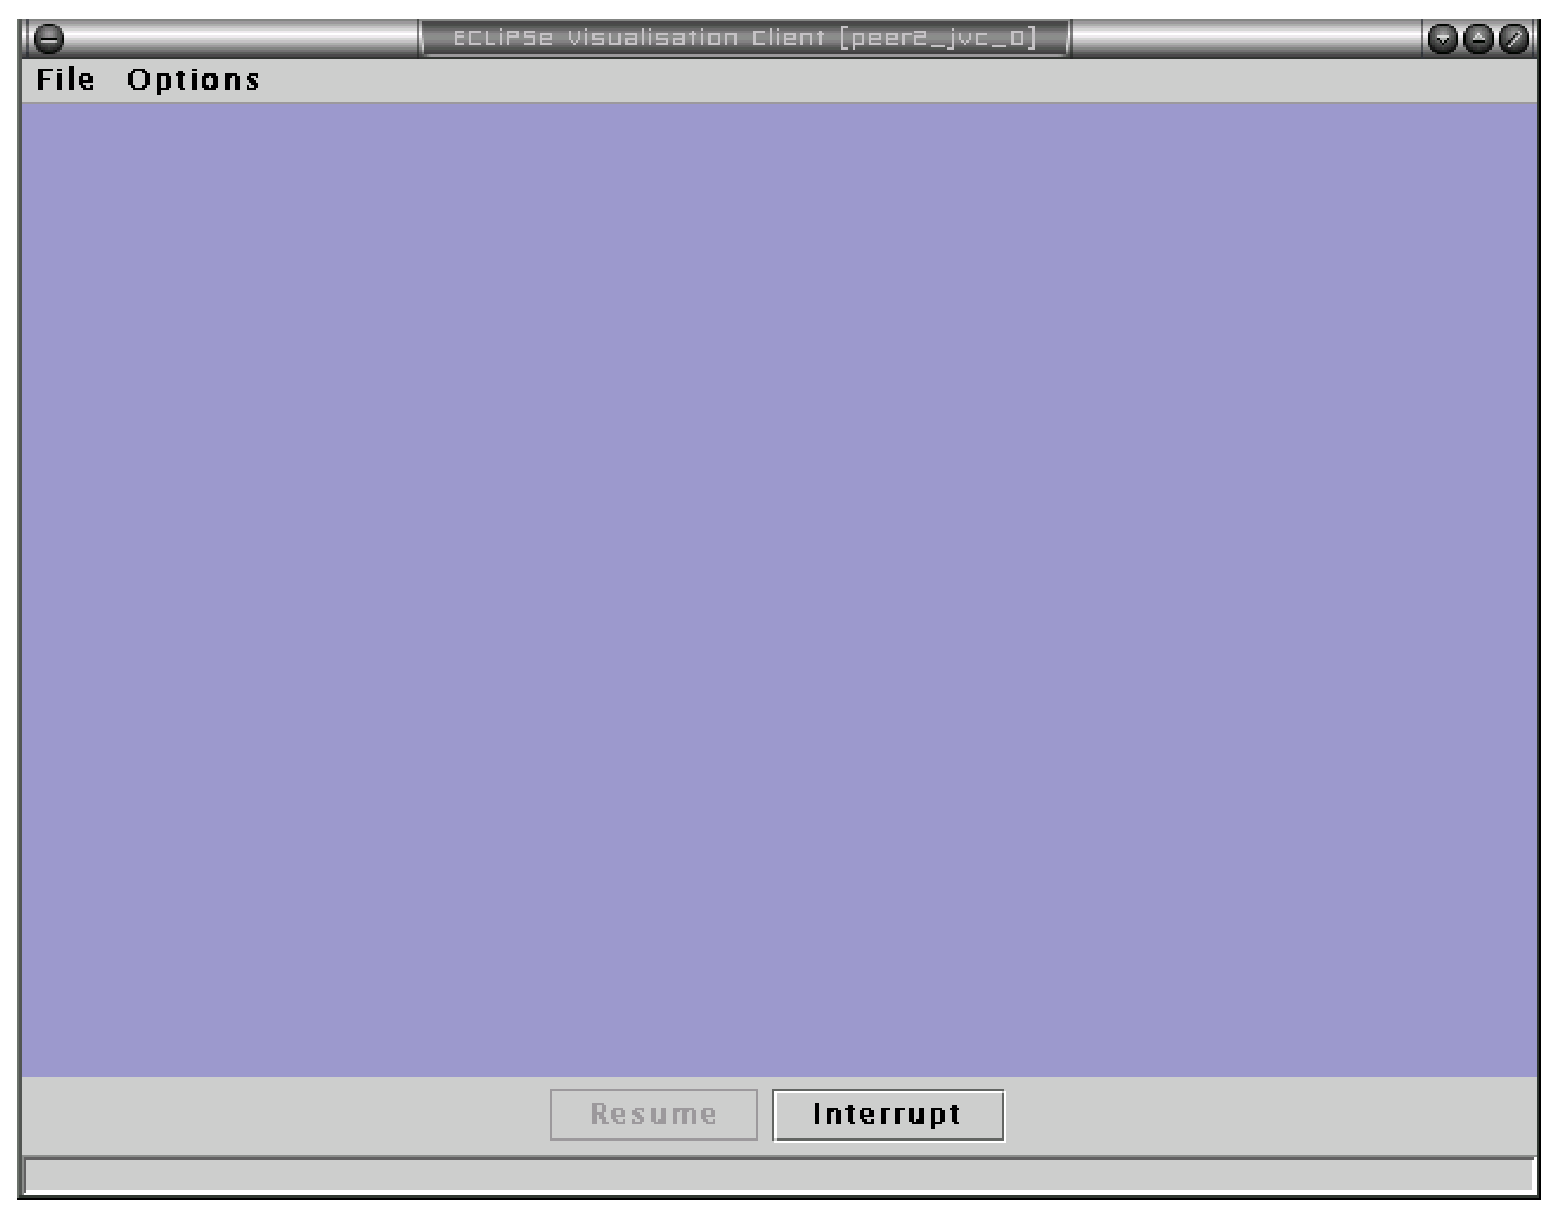
\includegraphics[width=8cm]{vcstartup}
\caption{The initial Java VC screen before any viewables have been created.}
\label{fig:startup}
\end{figure}


\section{Control}

When running a visualisation-annotated {\eclipse} program with a Java
VC attached, control of the {\eclipse} process may pass between
{\eclipse} and the VC throughout the program run.  That is to say at
certain key events in the program, {\eclipse} will pause in its
running of the program and wait for user interaction with the VC
before continuing.  In such circumstances, the VC is said to
\emph{hold} the control.

Table \ref{tab:events} details the default behaviour for each of the
visualisation events which may occur, and indicates whether or not
this default behaviour can be altered.

\begin{table}[htsp]
\label{tab:events}
\begin{tabular}{|l|p{7cm}|l|l|}
\hline
Event & Triggered by & Default hold & Alterable \\
\hline
\hline
viewable creation &
\viewablecreatetwo{} \viewablecreatethree{} \viewablecreatefour{} &
yes &
no \\
\hline
viewable expansion &
\viewableexpandthree{} \viewableexpandfour{} &
no &
yes \\
\hline
viewable contraction &
Backtracked over a viewable expansion &
no &
yes \\
\hline
viewable destruction &
Backtracked over a viewable creation &
yes &
yes \\
\hline
forward update &
One or more elements in a viewable have been updated, ie. had their
domain reduced or have been instantiated &
no &
yes \\
\hline
backward update &
A forward update has been backtracked over &
no &
yes \\
\hline
\end{tabular}
\caption{VC default behaviour for visualisation event.}
\end{table}

Should the VC hold, control can be passed back to {\eclipse} by
pressing the \textbf{Resume} button at the bottom of the VC window, or
by setting the \textbf{auto resume} timer.  The \textbf{Resume} button
and the \textbf{auto resume} timer are disabled when {\eclipse} has
control, see Figure \ref{fig:autoresume}.

\begin{figure}[htsp]
\centering
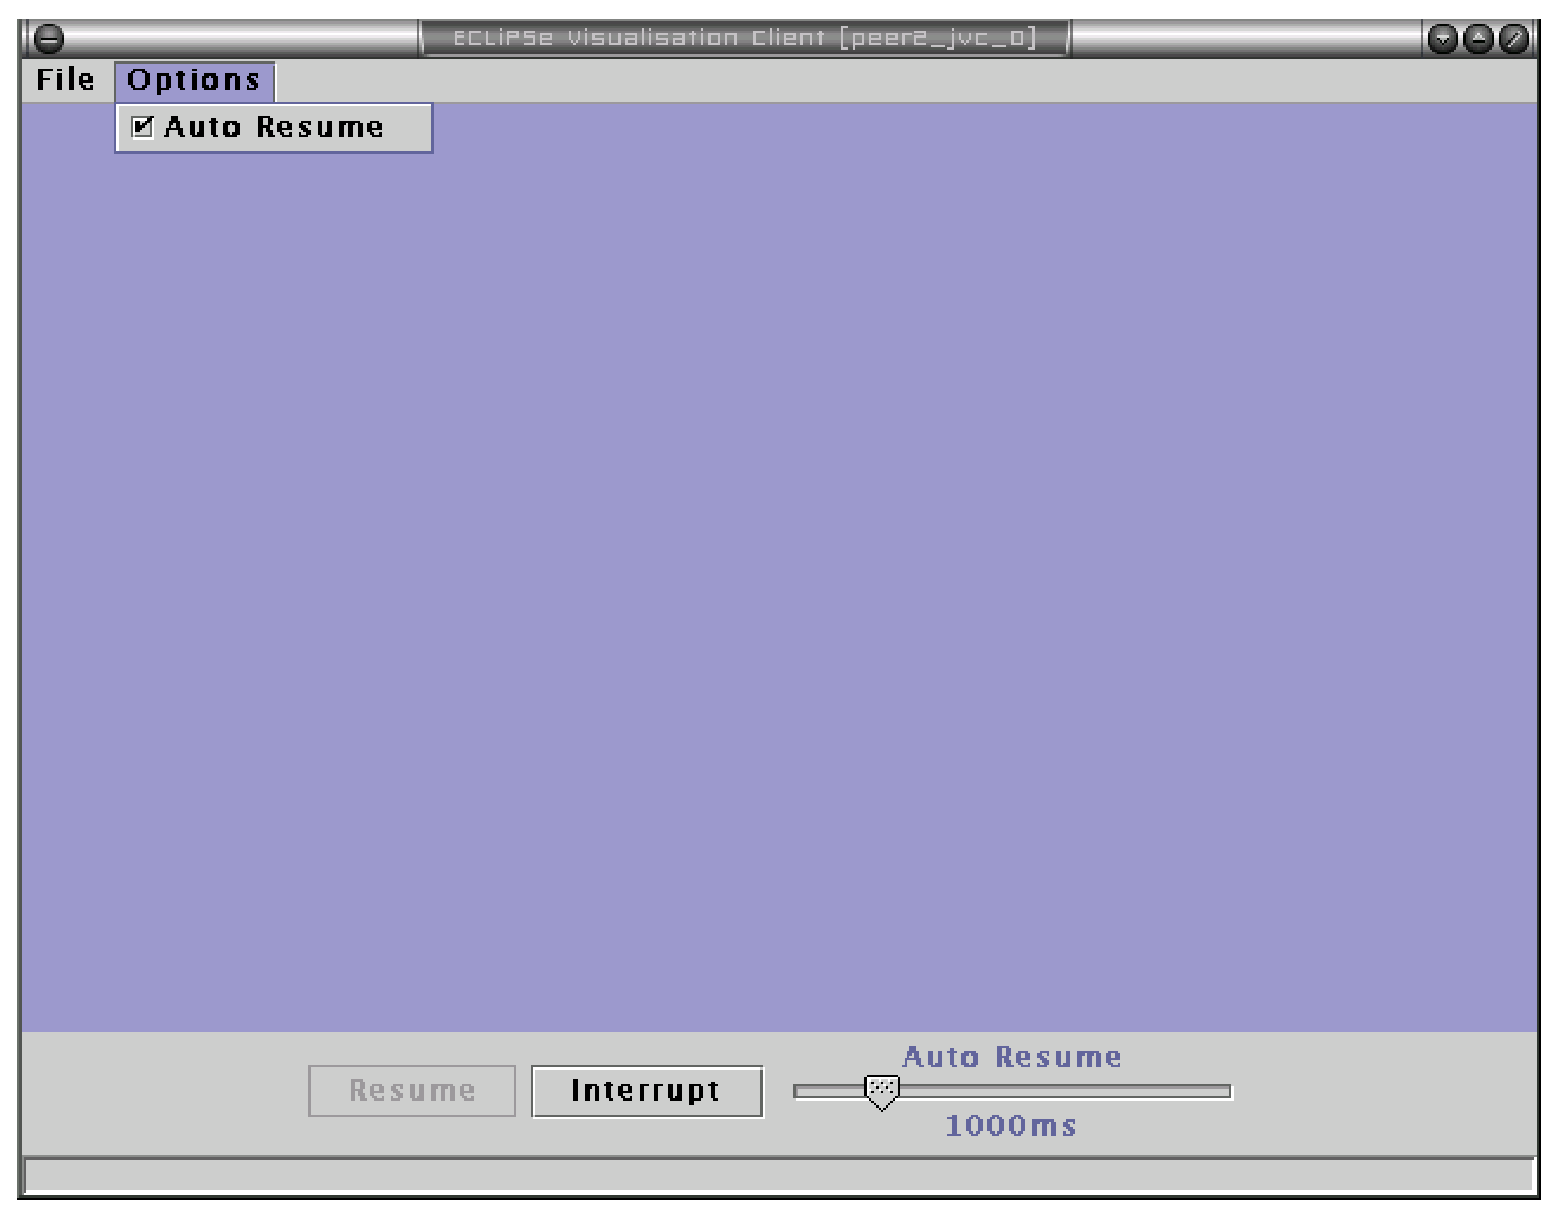
\includegraphics[width=8cm]{vcautoresume}
\caption{The VC showing the auto resume menu option and timer slider.}
\label{fig:autoresume}
\end{figure}


\section{Viewlets}

The Java VC provides many ways of visualising any single element of a
\viewable{}.

\begin{enumerate}
\item Textually, as though the element had been printed with
\bipref{write/1}{../bips/kernel/ioterm/write-1.html}.  This is
suitable for all \viewable{} types.
\item As a rectangular bar on a scale representing the current bounds
of a \emph{numeric_bounds} type \viewable{} element.  Bounds
\viewlet{}s can be aligned either vertically or horizontally.
\item As a node in a graph, similar to the simple textual
representation but enclosed in a geometric shaped node.
\item As an edge in a graph, with the textual representation attached
as a label to the edge.
\item With a colour which varies in shade and hue in response to
events occurring on the variable.
\end{enumerate}

When rendered on the screen these representations are referred to as
\viewlet{}s.  Figure \ref{fig:viewlets} shows the same variable
rendered using a number of \viewlet{} types.

\begin{figure}[htsp]
\centering
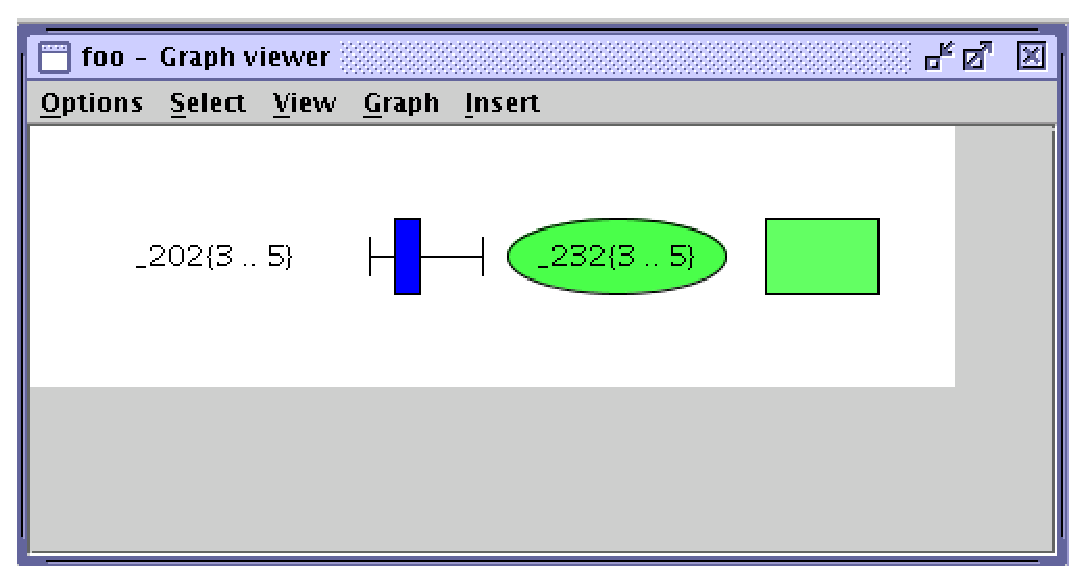
\includegraphics[width=6cm]{vcviewlets}
\caption{The FD variable with initial domain 0..10, reduced to 3..5 as
rendered by text, bound, node and fade \viewlet{}s.}
\label{fig:viewlets}
\end{figure}


\section{Viewers}

The Java VC currently contains five different methods for rendering
an entire \viewable{}.  Each of these methods can be thought of as a
window looking onto the \viewable{} and is referred to as a \viewer{}.

Upon a \viewable{} being created, the user is presented with a dialog
box asking which of the available \viewer{}s they wish to view the
\viewable{} with.

The currently available viewers are
\begin{description}
\item[TextTable] Renders any type of 1D and 2D \viewable{}s as a grid
of textual descriptions of the elements.
\item[BoundsTable] Renders numeric_bounds 1D and 2D \viewable{}s as a
grid of rectangles representing the size of the numeric domains.
\item[FadeTable] Renders 1D and 2D \viewable{}s as a grid of coloured
rectangles whose colour changes represent domain changes in the
\viewable{} elements.
\item[Desktop] Allows the user to place all available representations
of the \viewable{} elements anywhere on a desktop window.  Also
enables the loading of an arbitrary background image from file, and for
placing images alongside \viewlet{}s.
\item[Network] Renders \texttt{graph(fixed)} \viewable{}s graphically
as connected nodes, where the textual representation of the
\viewable{} elements is displayed at nodes and along edges.
\item[Network (0/1)] Similar to the Network viewer except that if the
edge annotation can be interpreted as the number 0, then the edge is
not drawn.  If it can be interpreted as the number 1, it is drawn in
black.  Any other value has the edge draw in gray.
\item[Network (Capacity)] Similar to the Network viewer except that
the edge labels are interpreted as fractions indicating the capacity
of a link in a flow network.  0.0 indicating unused (thin black line)
up to 1.0 indicating full usage (thick black line) and any number
greater than one indicating over utilisation (very think red line).
If the edge data cannot be interpreted as a number (eg. it is a
variable) it is assumed to be 0.
\item[Gantt] Interprets the first three rows of any 2D viewable with
\texttt{numeric_bounds} elements (and at least 3 rows) as being the
start times, durations and resource requirements of a scheduling
problem.  The resulting schedule/partial schedule is rendered as a
gantt chart.
\item[Bar chart] Renders any $n$-dimensional \texttt{numeric_bounds}
viewable as a bar chart.  Extra dimensions will be separated by gaps
in the chart.
\end{description}

\begin{figure}[htsp]
\centering
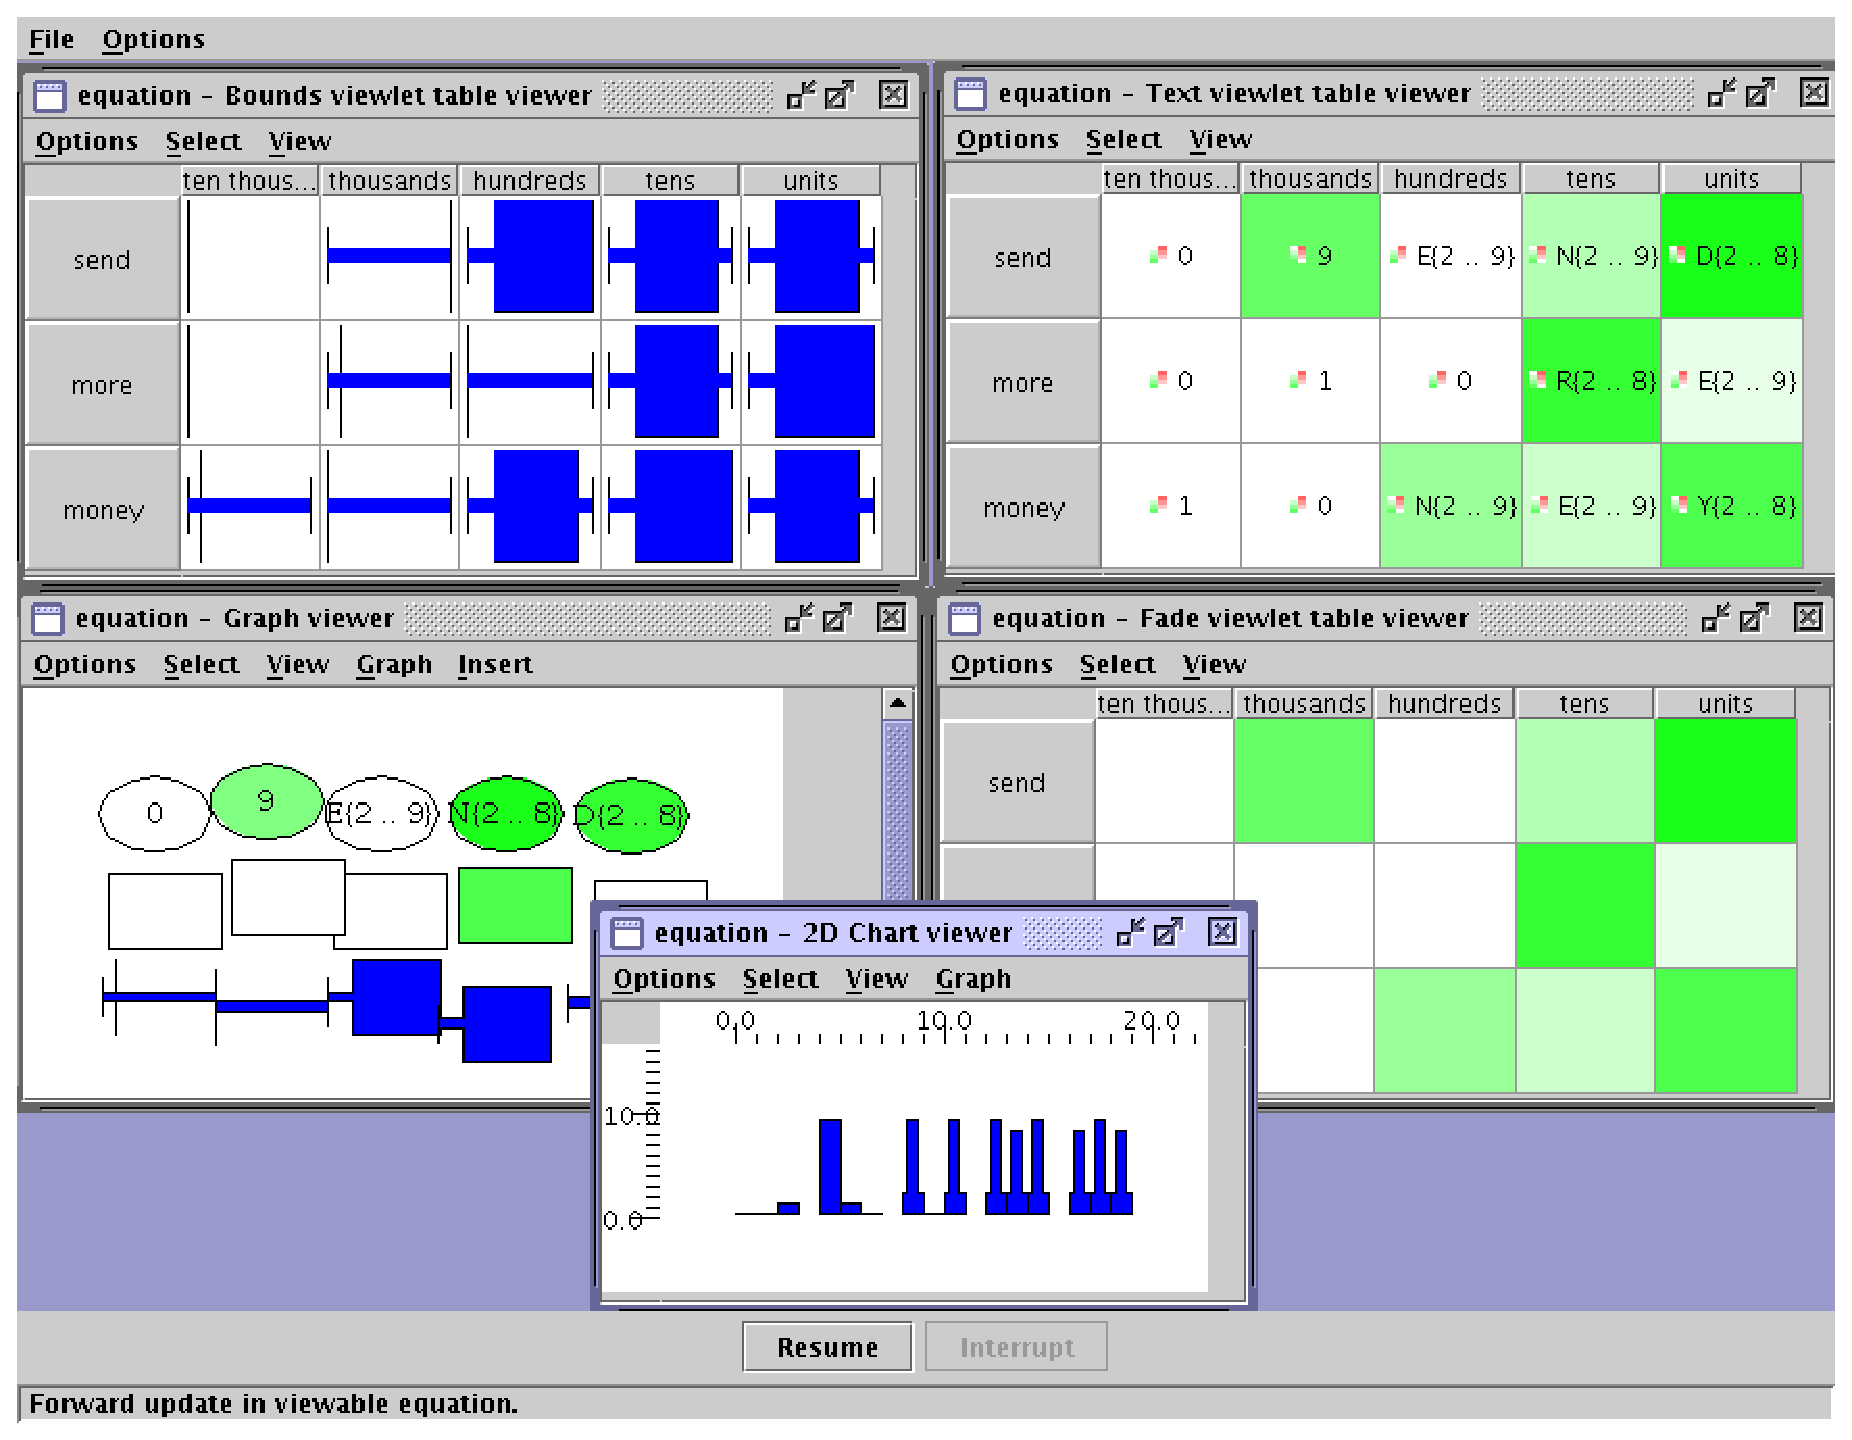
\includegraphics[width=11cm]{vcallviewers}
\caption{The VC showing some of the applicable viewers for the \texttt{SEND+MORE=MONEY} example.}
\label{fig:allviewers}
\end{figure}

\begin{figure}[htsp]
\centering
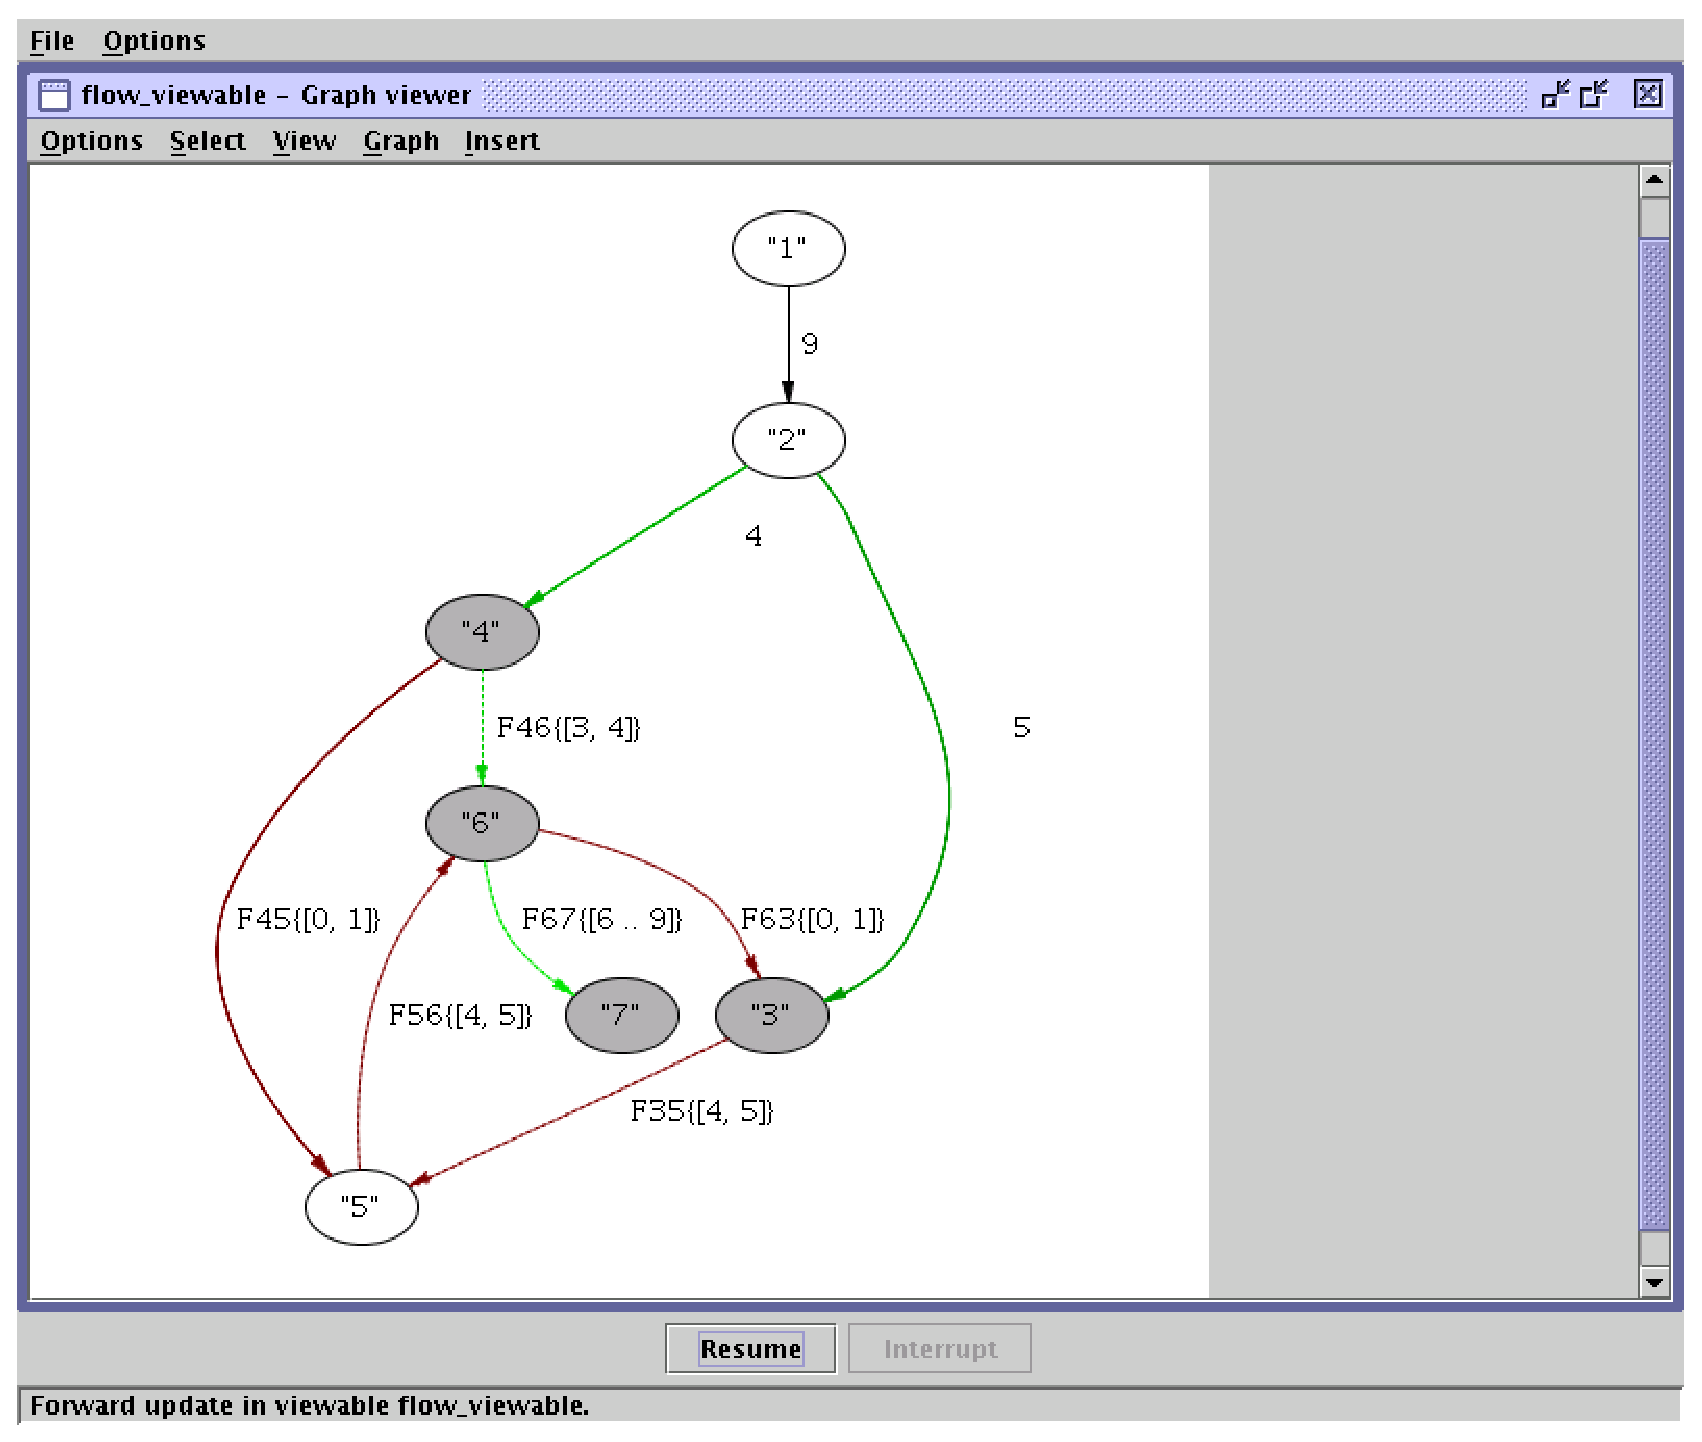
\includegraphics[width=10cm]{vcnetworkviewer}
\caption{The VC showing the network viewer displaying the graph example.}
\label{fig:networkviewer}
\end{figure}

\begin{figure}[htsp]
\centering
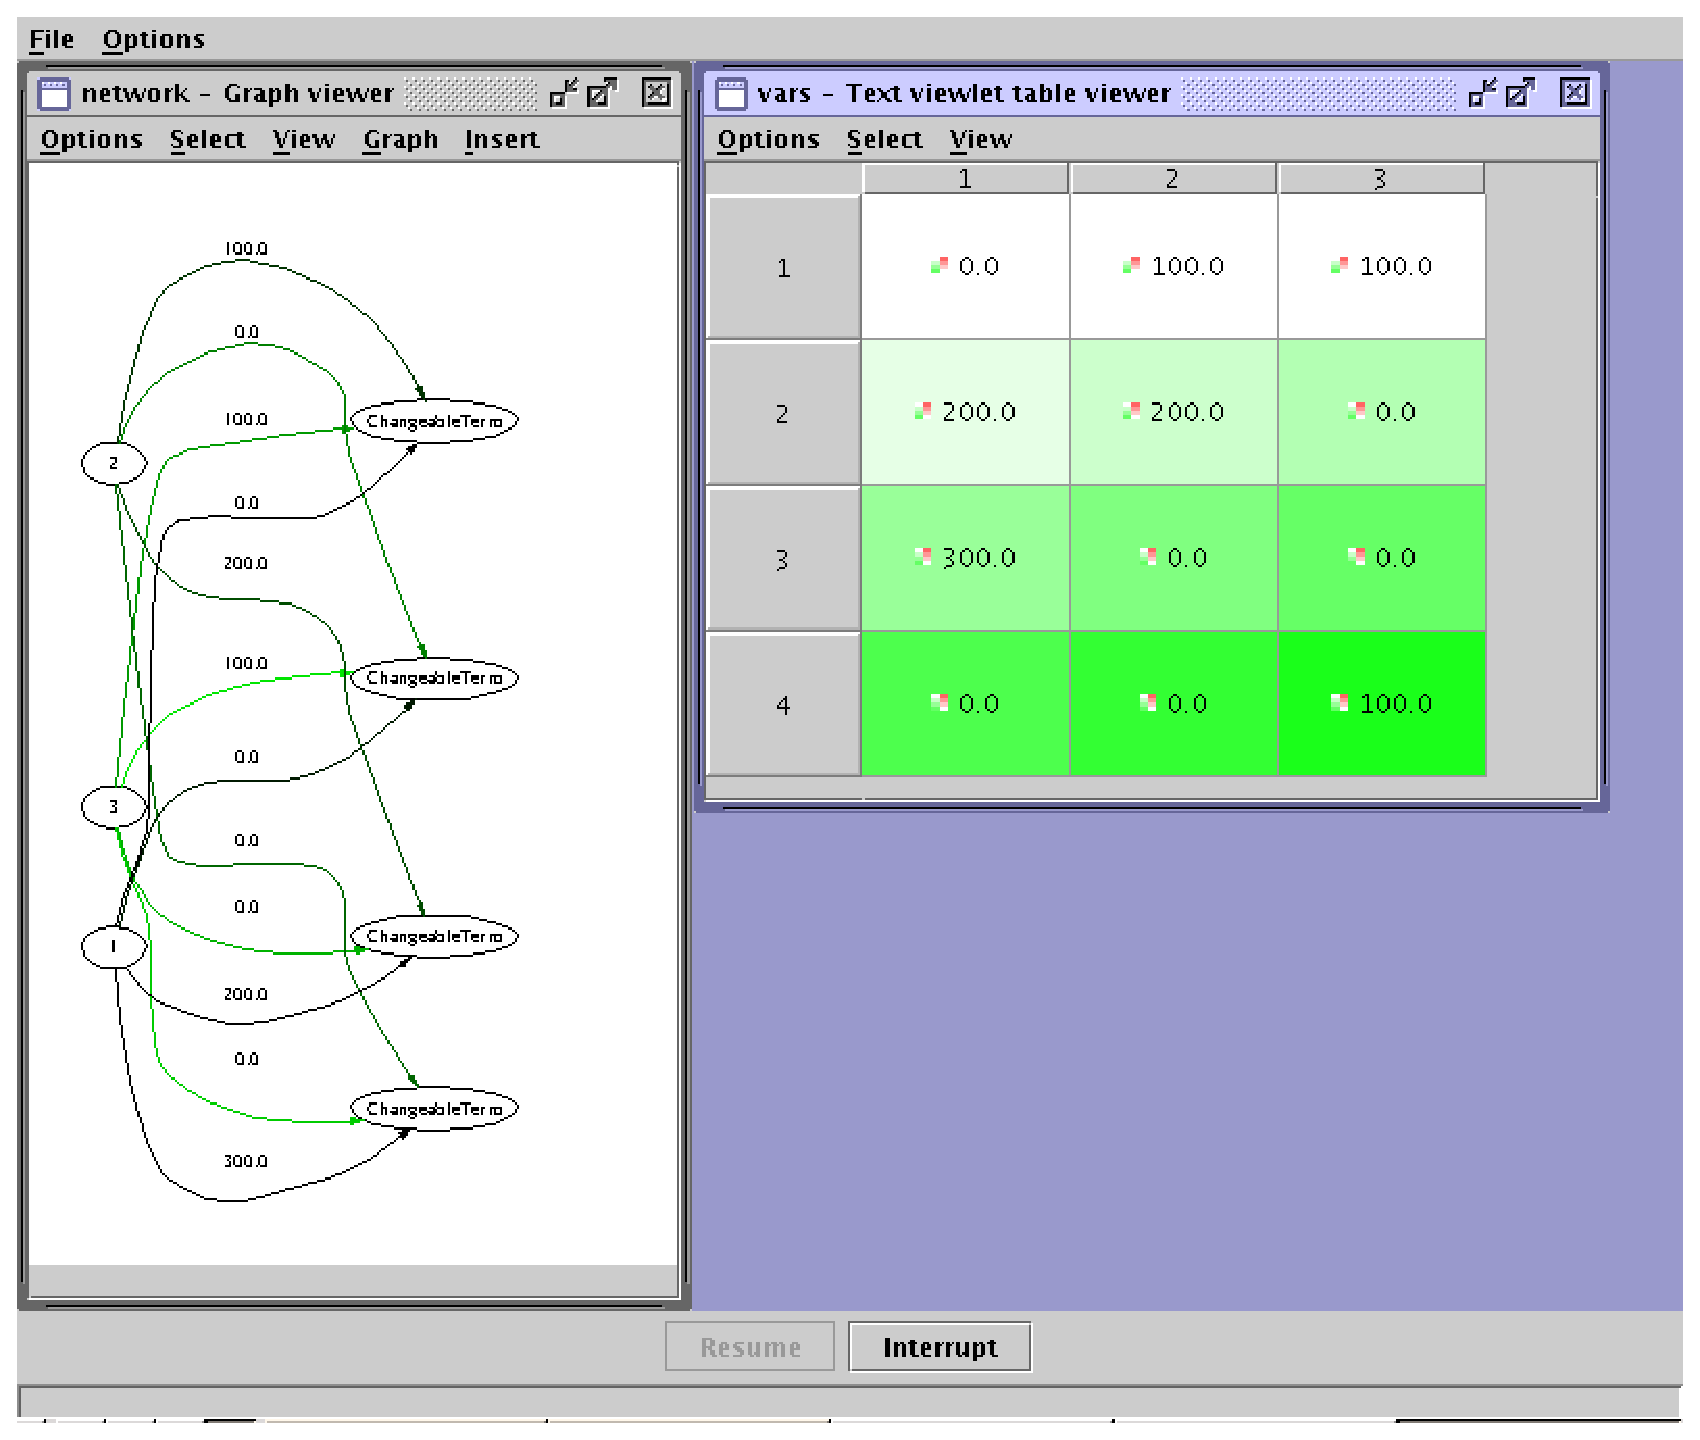
\includegraphics[width=10cm]{vcchangeableexample}
\caption{The VC showing various viewers for the changeable solver example.}
\label{fig:changeableexample}
\end{figure}

Common to all viewers are the three menus \textbf{Options},
\textbf{Select} and \textbf{View}, the latter two also being
accessible by pressing the right mouse button.

\subsection{Options menu}
The options menu contains controls for \viewer{}-wide properties.
\begin{description}
\item[Hold at expansions] Determines whether this \viewer{} will hold
control when the \viewable{} is expanded.
\item[Hold at contractions] Determines whether this \viewer{} will hold
control when the \viewable{} is contracted.
\item[Hold at destruction] Determines whether this \viewer{} will hold
control when the \viewable{} is destroyed.  This option is useful for
examining the state of the \viewable{} immediately before the
creation is backtracked over.
\item[View propagation steps] Controls how frequently the visualisation client is informed of \emph{forward update} events.

  \begin{description}
  \item[fine] Events are sent as soon as they occur.
  \item[coarse] Events are sent at priority 8 in the {\eclipse}
  program.  Typically this means that all the propagation that occurs
  as a result of a single user level search step are sent together.
  \item[timed] Events are collected and sent at regular timed
  intervals.
  \end{description}

\item[Track updates] When set, the \viewer{} will attempt to ensure
that all updates are visible within the window.  This can be important
when visualising large \viewable{}s which may not easily fit the
window.
\end{description}

Figure \ref{fig:optionsmenu} shows the default settings for the
\textbf{Options} menu.  Note that the \textbf{View propagation steps}
options are disabled because {\eclipse} has control and the update
granularity can only be changed when the Java VC is holding control.

\begin{figure}[htsp]
\centering
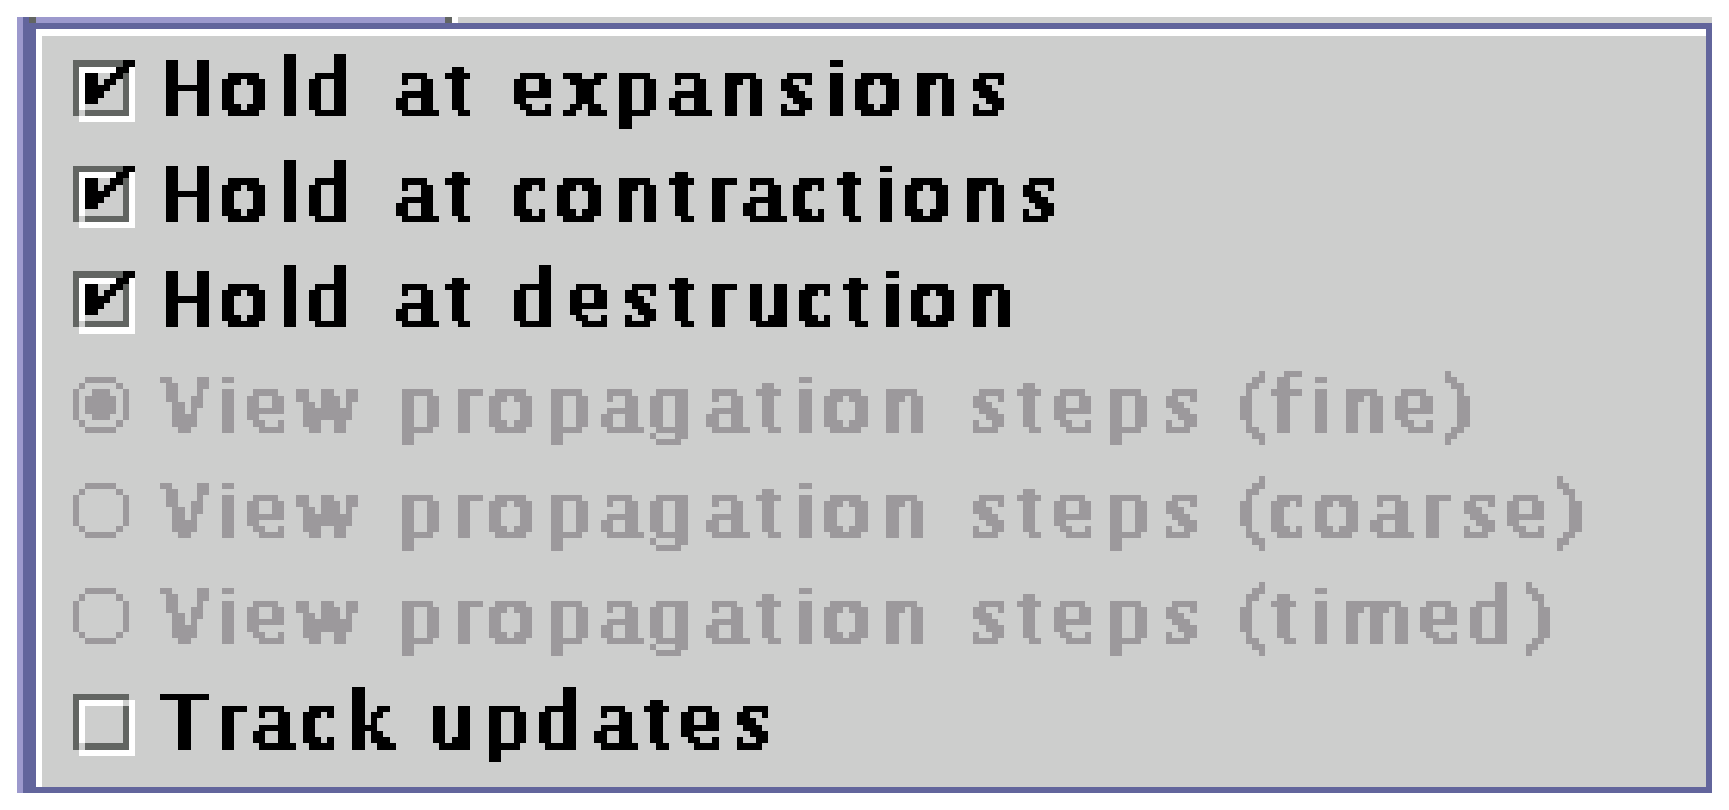
\includegraphics[width=4cm]{vcoptionsmenu}
\caption{The options menu, common to all viewers.}
\label{fig:optionsmenu}
\end{figure}

\subsection{Select menu}
Contains convenience commands for dealing with the currently selected
set of \viewlet{}s.

Selecting individual \viewlet{}s can be done clicking on them with the left mouse button, whilst selecting ranges can be done by dragging the mouse across a range of \viewlet{}s.

\begin{description}
\item[Select all viewlets] Sets the selection to the entire \viewable{}.
\item[Select updating viewlets(s)] Sets the selection to only those
\viewlet{}s which have been marked as updating (either \emph{forward}
or \emph{backward}).  This option is only enabled when the Java VC has
control, since it requires the state of the viewables to remain
constant during the selection process.
\item[Clear selection] Clears the selection.
\end{description}


\begin{figure}[htsp]
\centering

\includegraphics[width=3.5cm]{vcselectmenu}
\caption{The select menu, common to all viewers.}
\label{fig:selectmenu}
\end{figure}

\subsection{View menu}

So as to facilitate visualisation of large \viewable{}s, all \viewer{}s
have the ability to zoom in and out.  All the options are self
explanatory and will not be expanded further upon except to mention
that the \textbf{Zoom to fit width} and \textbf{Zoom to fit height}
options operate on the whole \viewer{} and not just the selected
\viewlet{}s.

\begin{figure}[htsp]
\centering
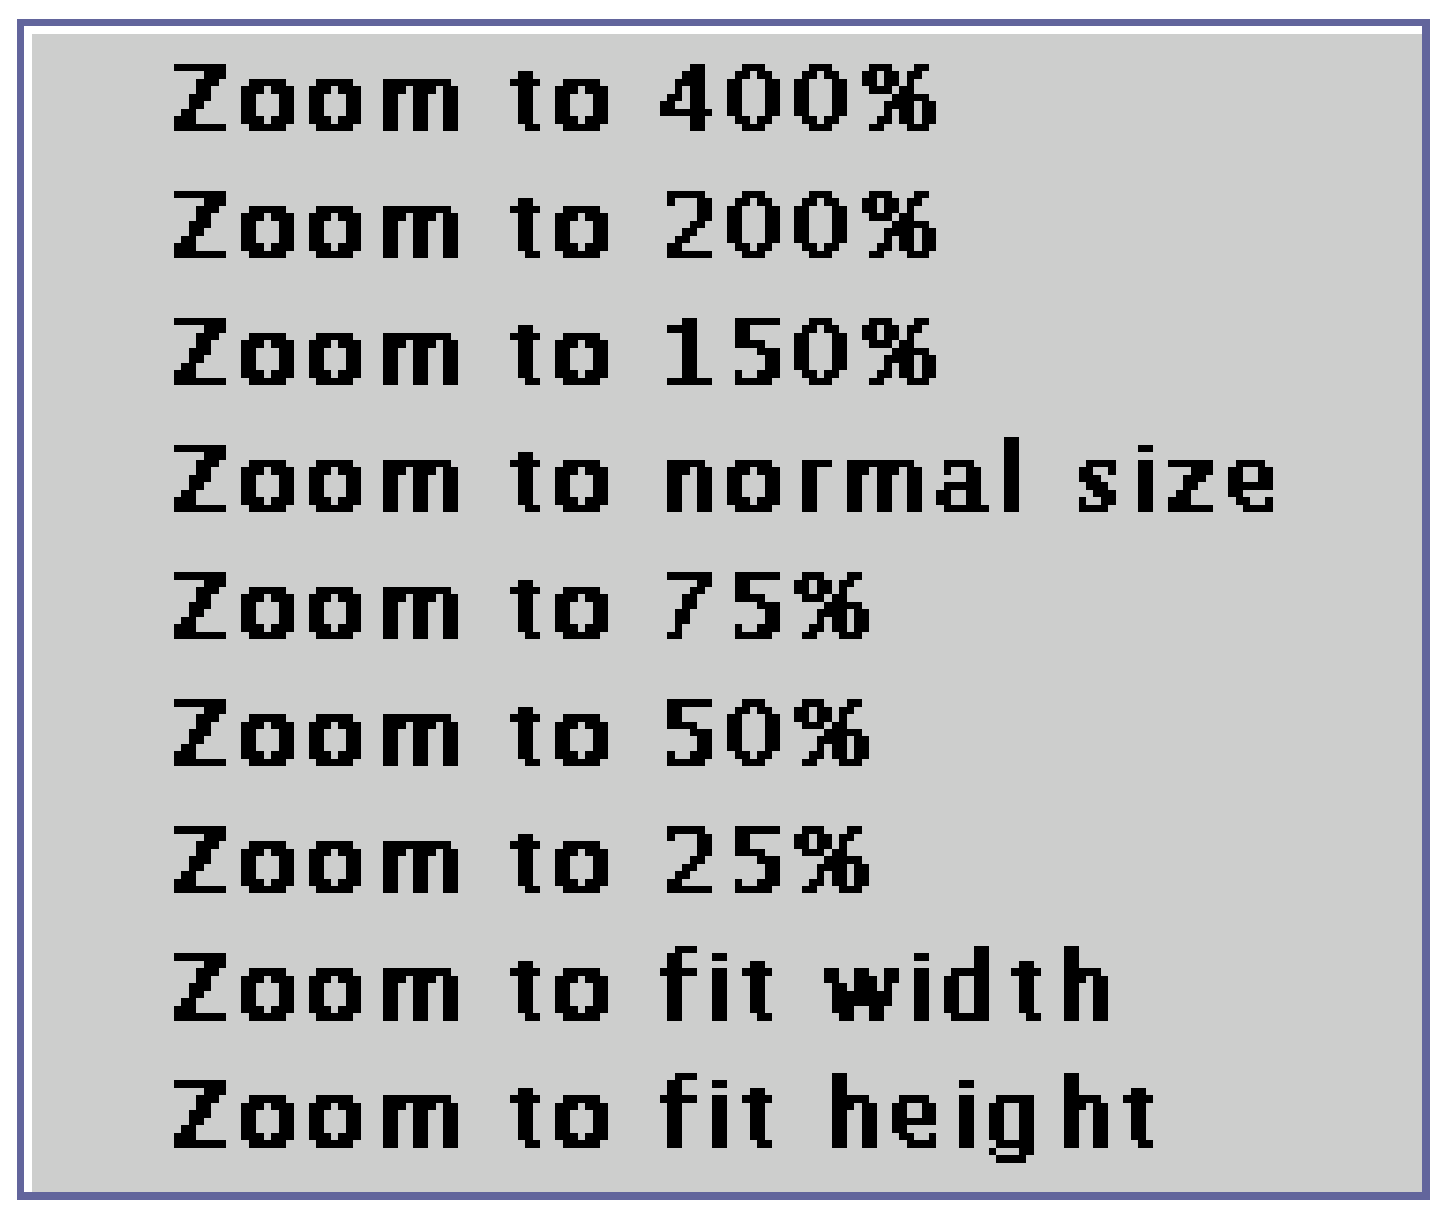
\includegraphics[width=3.5cm]{vcviewmenu}
\caption{The view menu, common to all viewers.}
\label{fig:viewmenu}
\end{figure}

Both the network and desktop viewers have an extra item on the view
menu, \emph{Toggle high quality}.  This toggles between quick
rendering and high quality views, and may help to make the VC more
reactive under high load.

\subsection{Viewlet actions}

Within a \viewer{}, as previously mentioned, any number of \viewlet{}s
may be selected.  These \viewlet{}s, once selected can have actions
performed on them.  The actions are selected by pressing the right
mouse button in order to bring up the context sensitive actions menu.
If the \viewlet{}s in the selection are of different types then all
the available actions are displayed and once one has been selected, it
will be applied to all applicable \viewlet{}s in the selection.  This
is a change from previous versions of the visualisation client, which
would display only those actions common to all \viewlet{}s.

\subsubsection{Hold on update}
The most common action, which can be performed on any type of
\viewlet{} is the \emph{Hold on updates} action, which, when set,
indicates that the Java VC should hold control whenever any sort of
update event is issued for the corresponding \viewable{} element.  The
\emph{Hold on updates} property of a \viewlet{} is indicated by a
slight ``greying'' out of the \viewlet{}, or in the case of
\viewlet{}s attached to edges in the network viewer, the edge is drawn
``dotted'' instead of solid.

Figure \ref{fig:viewlethold} shows the graphical effect of setting the
\emph{Hold on update} property of a text \viewlet.

\begin{figure}[htsp]
\centering
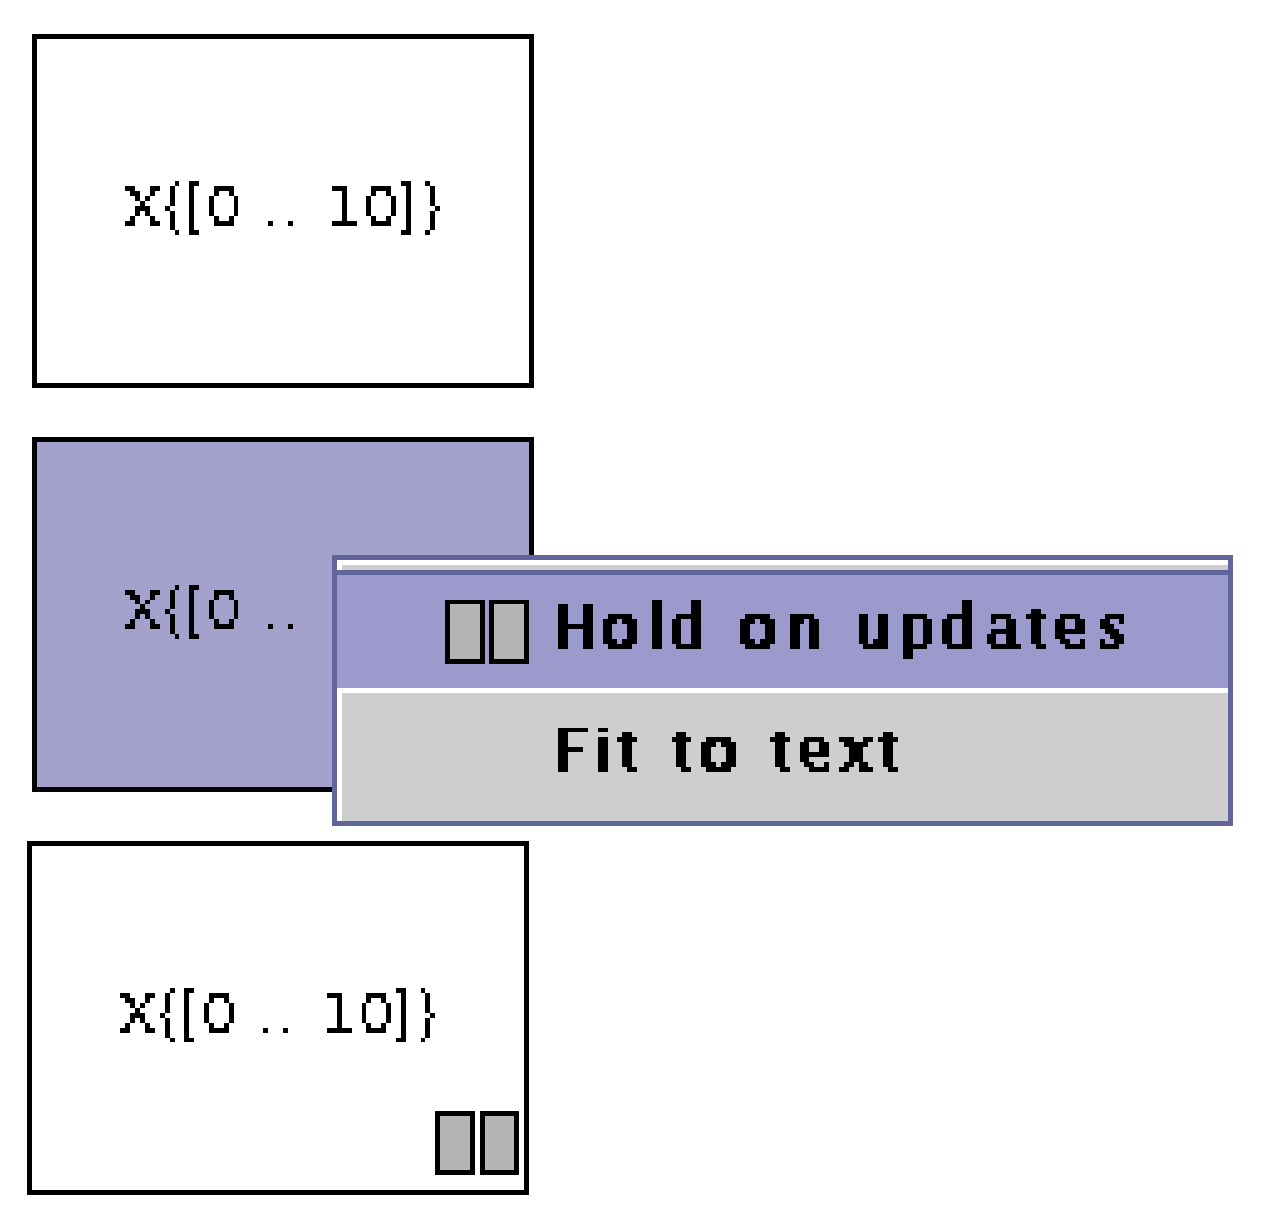
\includegraphics[width=4cm]{vcviewlethold}
\caption{The sequence of actions required to select \textbf{Hold on update} for a \viewlet{}}
\label{fig:viewlethold}
\end{figure}

Table \ref{tab:viewletactions} lists the available \viewlet{} actions
and indicates for which type the actions are valid.

\begin{table}[htsp]
\centering
\begin{tabular}{|l|p{7cm}|l|}
\hline
Name & Description & Applicable \\
\hline
\hline
Hold on updates & Causes the VC to hold control on forward or backward
update events for the selected \viewlet{}s. & all \\

% \hline
% Fit to text & Resizes the selected \viewlet{}s to exactly fit the
% width of the widest textual representation.  In order to resize
% \viewlet{}s in a \textbf{TextTableLight} you should simply resize the
% column by clicking on the edge of the column header and dragging, then
% the whole column will resize. & 1+ & 0 \\

\hline
Fade update history & Toggles using the background color of the
viewlet to indicate recent update history.  This has the effect of
fading from green to white in the event of a forward update and from
red to white for backward updates. & text, node, fade, edge \\

\hline
View bounds in detail & Pops up a window detailing the original bounds and the current bounds for the single selected \viewlet{}. & bound \\

\hline
Align bounds & Causes the selected \viewlet{}s to use the same underlying scale when displaying the bounds.  This allows variables whose initial bounds were different to be visually compared. & bound \\

\hline
Toggle horizontal/vertical range bar & Toggles the rotation of the bar for all bounds \viewlet{}s & bound \\
\hline
\end{tabular}
\caption{The available \viewlet{} actions and associated types.}
\label{tab:viewletactions}
\end{table}

\subsection{Desktop/Network viewers}

All the \textbf{table} viewers have essentially the same functionality
-- they do not allow flexible placement of viewables and both deal
only with 1 or 2 dimensional \viewable{}s.  A more flexible \viewer{}
is provided in the \textbf{Desktop viewer}.

This \viewer{} aims to implement the common \emph{desktop} metaphor by
providing the user with a rectangular region of the screen upon which
\viewlet{}s can be dropped, stacked and moved around as though they
were pieces of paper on a desk.

\subsubsection{Adding viewlets}
Typically, \viewlet{}s will be added to a desktop immediately after the
\viewer{} has been created.  To minimise the overhead of having to
layout the \viewlet{}s each time the user's program is run (a
potentially time consuming task), the Java VC provides an automatic
\emph{recording and repeat} mechanism which is triggered every time a
\viewer{} is created. Section \ref{sec:scenarios} explains this
feature in more detail.

Adding \viewlet{}s to a Desktop \viewer{} is done by selecting the
required \viewlet{} type from the \textbf{Insert} menu.  This menu
will contain only those \viewlet{} types which are appropriate for the
type of the \viewable{}.

Once an appropriate \viewlet{} type has been selected, the range
selection dialog will pop up, from which any combination of dimension
ranges may be selected.

Figure \ref{fig:rangeselect} shows the range select dialog for the on
going \texttt{SEND+MORE=MONEY} example.

\begin{figure}[htsp]
\centering
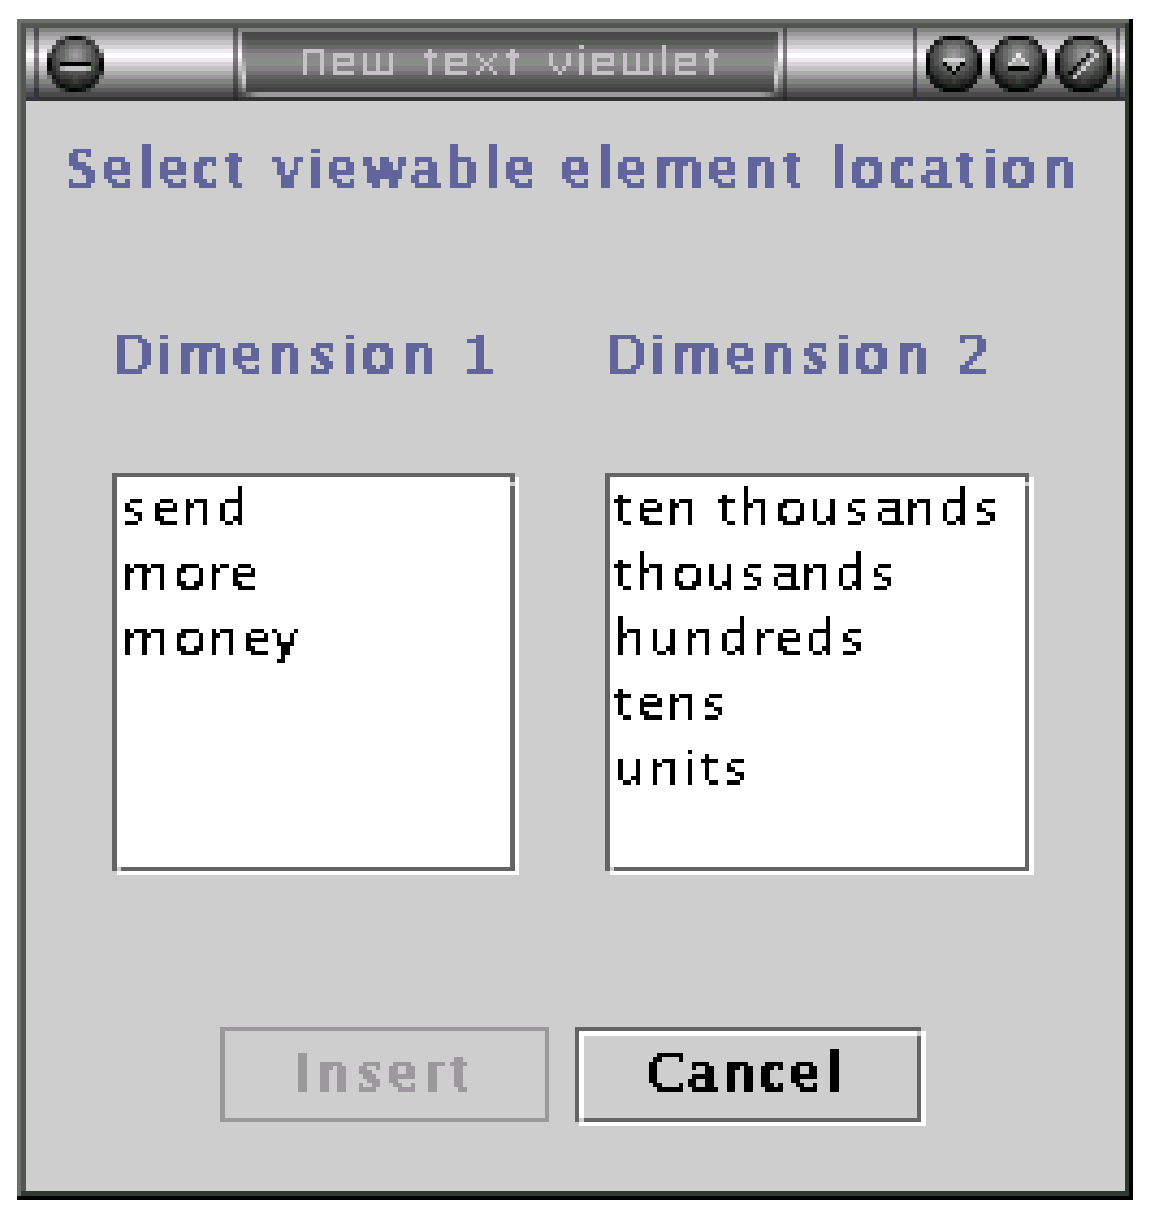
\includegraphics[width=4cm]{vcrangeselect}
\caption{The range selection dialog for the \texttt{SEND+MORE=MONEY} example}
\label{fig:rangeselect}
\end{figure}

At least one selection must be made from each of the dimensions,
though it is possible to select multiple values in each dimension.

Figures \ref{fig:rangeselect1d} and \ref{fig:rangeselect2d} illustrate
the default layout of \viewlet{}s when 1 and 2 dimensional ranges are
selected. The desktop will automatically resize to ensure that all
\viewlet{}s fit.  Attempts to move a viewlet \emph{off} the desktop
will cause it to grow.

\begin{figure}[htsp]
\centering
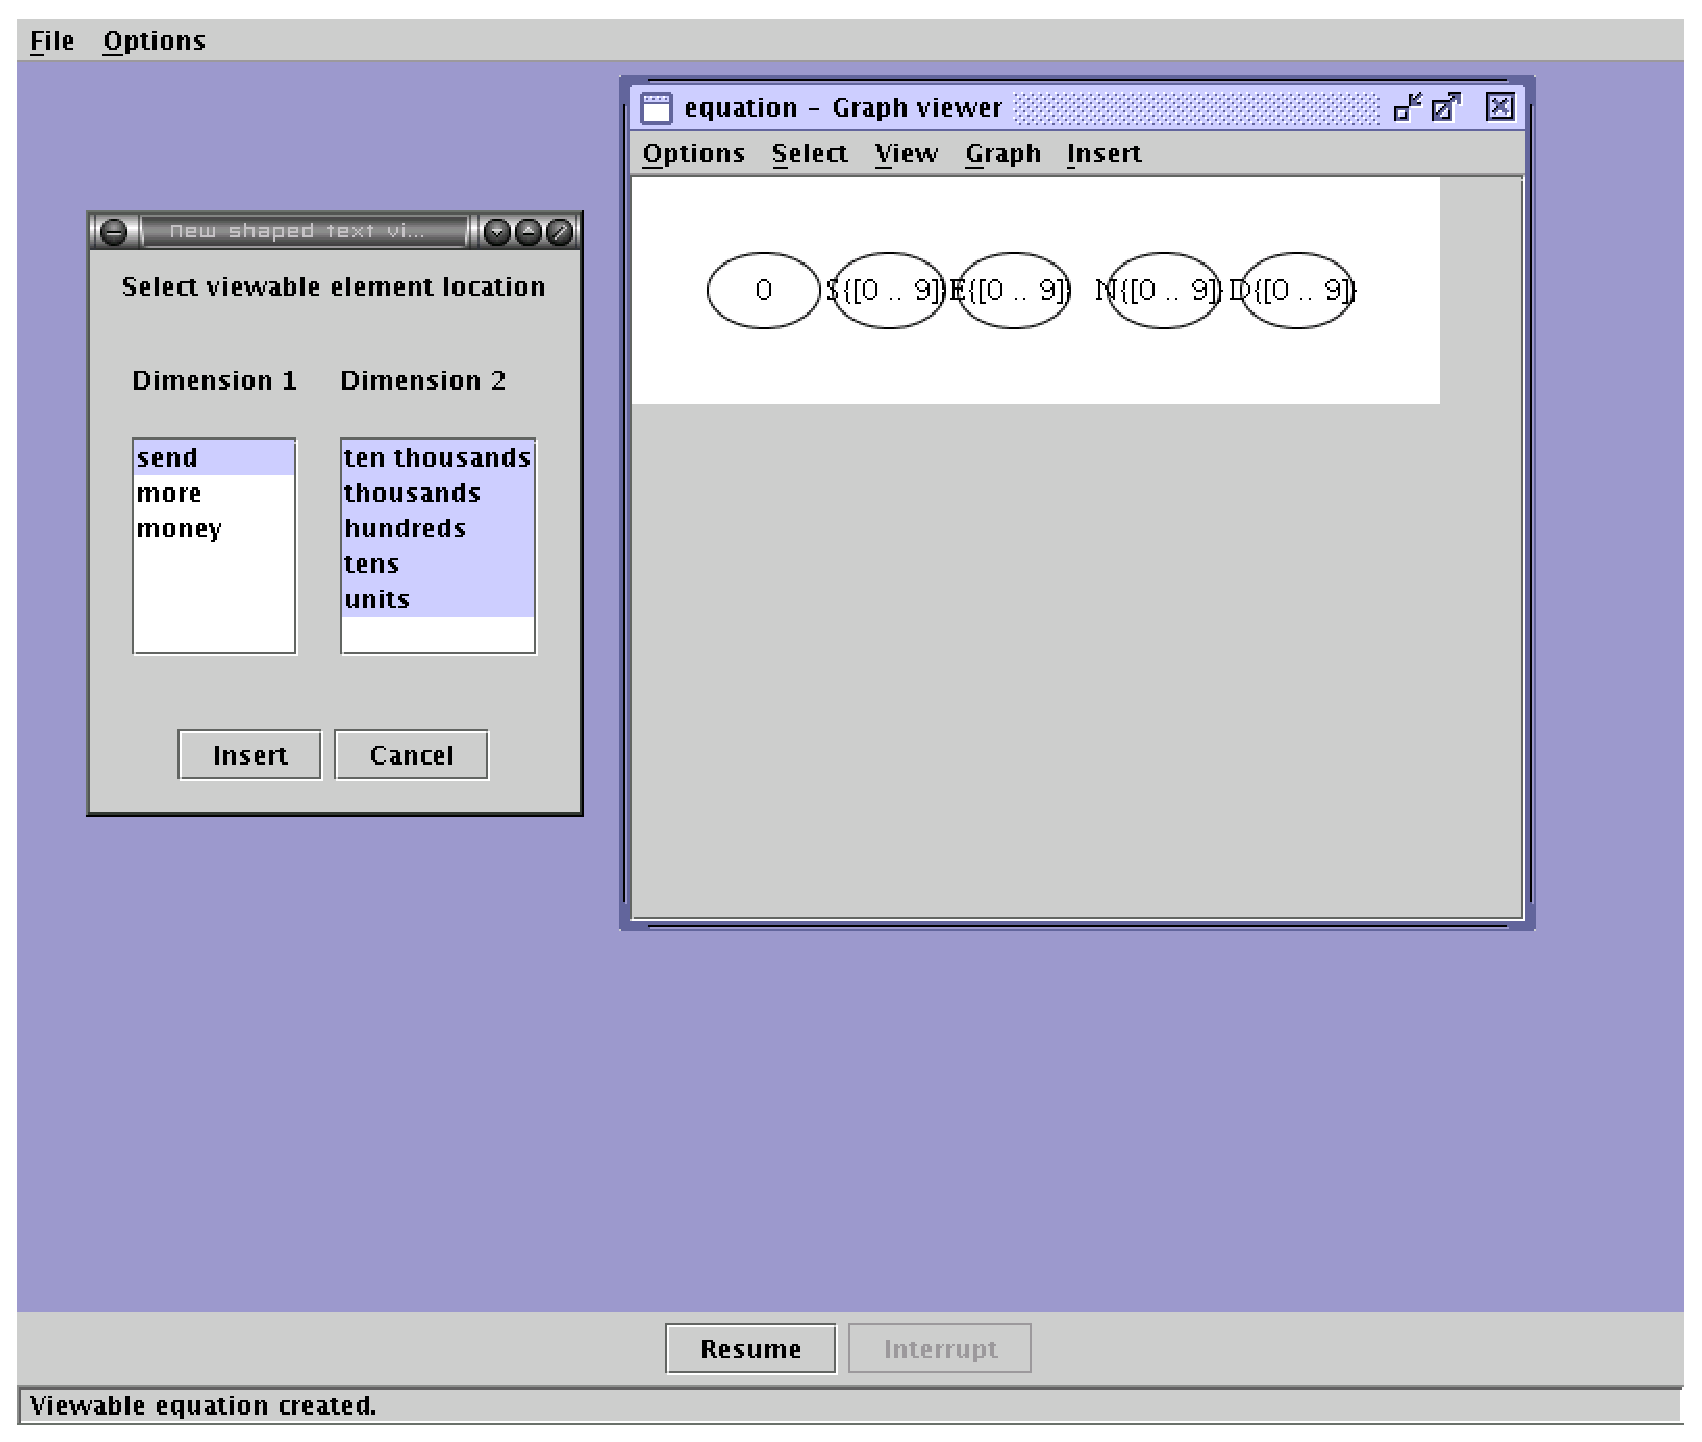
\includegraphics[width=10cm]{vcrangeselect1d}
\caption{The result of selecting a 1D range}
\label{fig:rangeselect1d}
\end{figure}

\begin{figure}[htsp]
\centering
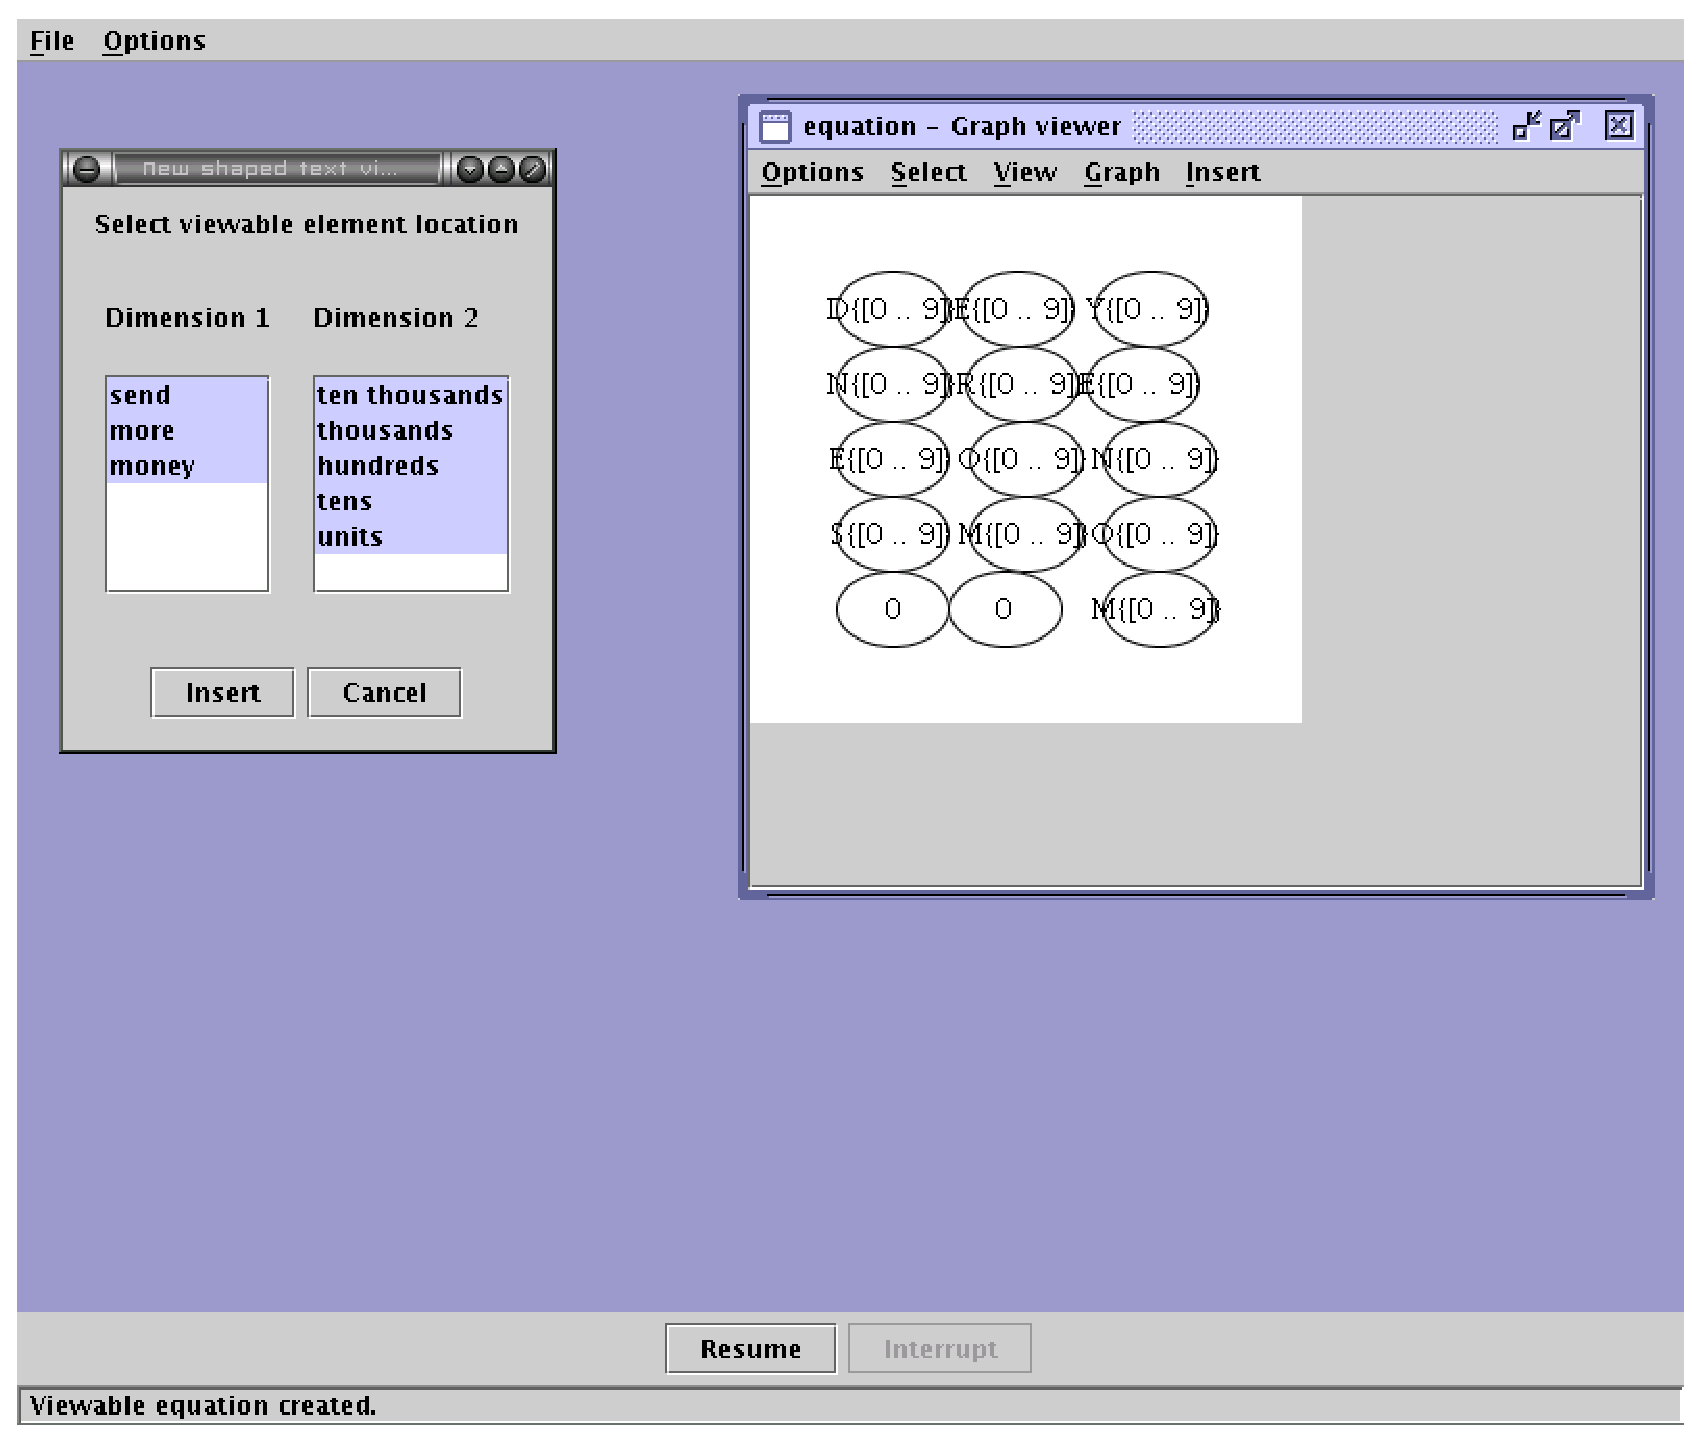
\includegraphics[width=10cm]{vcrangeselect2d}
\caption{The result of selecting a 2D range}
\label{fig:rangeselect2d}
\end{figure}

Higher dimension range selections result in a stacked 2D grid, with
progressive dimensions appearing underneath the initially visible grid.

\subsection{Adding images}

As well as \viewlet{}s, the \textbf{Desktop viewer} can show icons
loaded from disk by selecting the \textbf{Image} option from the
\textbf{Insert} menu.  This brings up a file selection dialog from
which the user may select an image file to load.  The loaded image
will be added to the \viewer{} as a small icon which is selectable and
movable like other items on the desktop.  Currently there is no way to
increase the size of the loaded image.

\subsubsection{Background images}
In keeping with the computer GUI \emph{desktop} metaphor, the user may
set the \emph{background} image for the desktop \viewer{}.  Aside from
making the \viewer{} look pretty this feature is intended to allow
graphical context to be associated with the visualisation of a program.
For example the background image could be a diagram representing the
network topology and the values being visualised could be the flows
through various parts of the network.  By placing the \viewlet{}s near
the appropriate nodes on the background image the user could more
easily visualise the network flow problem.

Background images are loaded by selecting the \textbf{Import
background image} option from the \textbf{Background} menu and are
removed by selecting the \textbf{Clear background} option.  Currently
only \textbf{GIF}, \textbf{PNG} and \textbf{JPEG} format images can be
loaded.

In keeping with our \texttt{SEND+MORE=MONEY} example, figure
\ref{fig:sendmoremoney} shows the problem visualised on a desktop
viewer, placed over a background image\footnote{Background image
\copyright 1999-2003 \texttt{www.barrysclipart.com}}.


\begin{figure}[htsp]
\centering
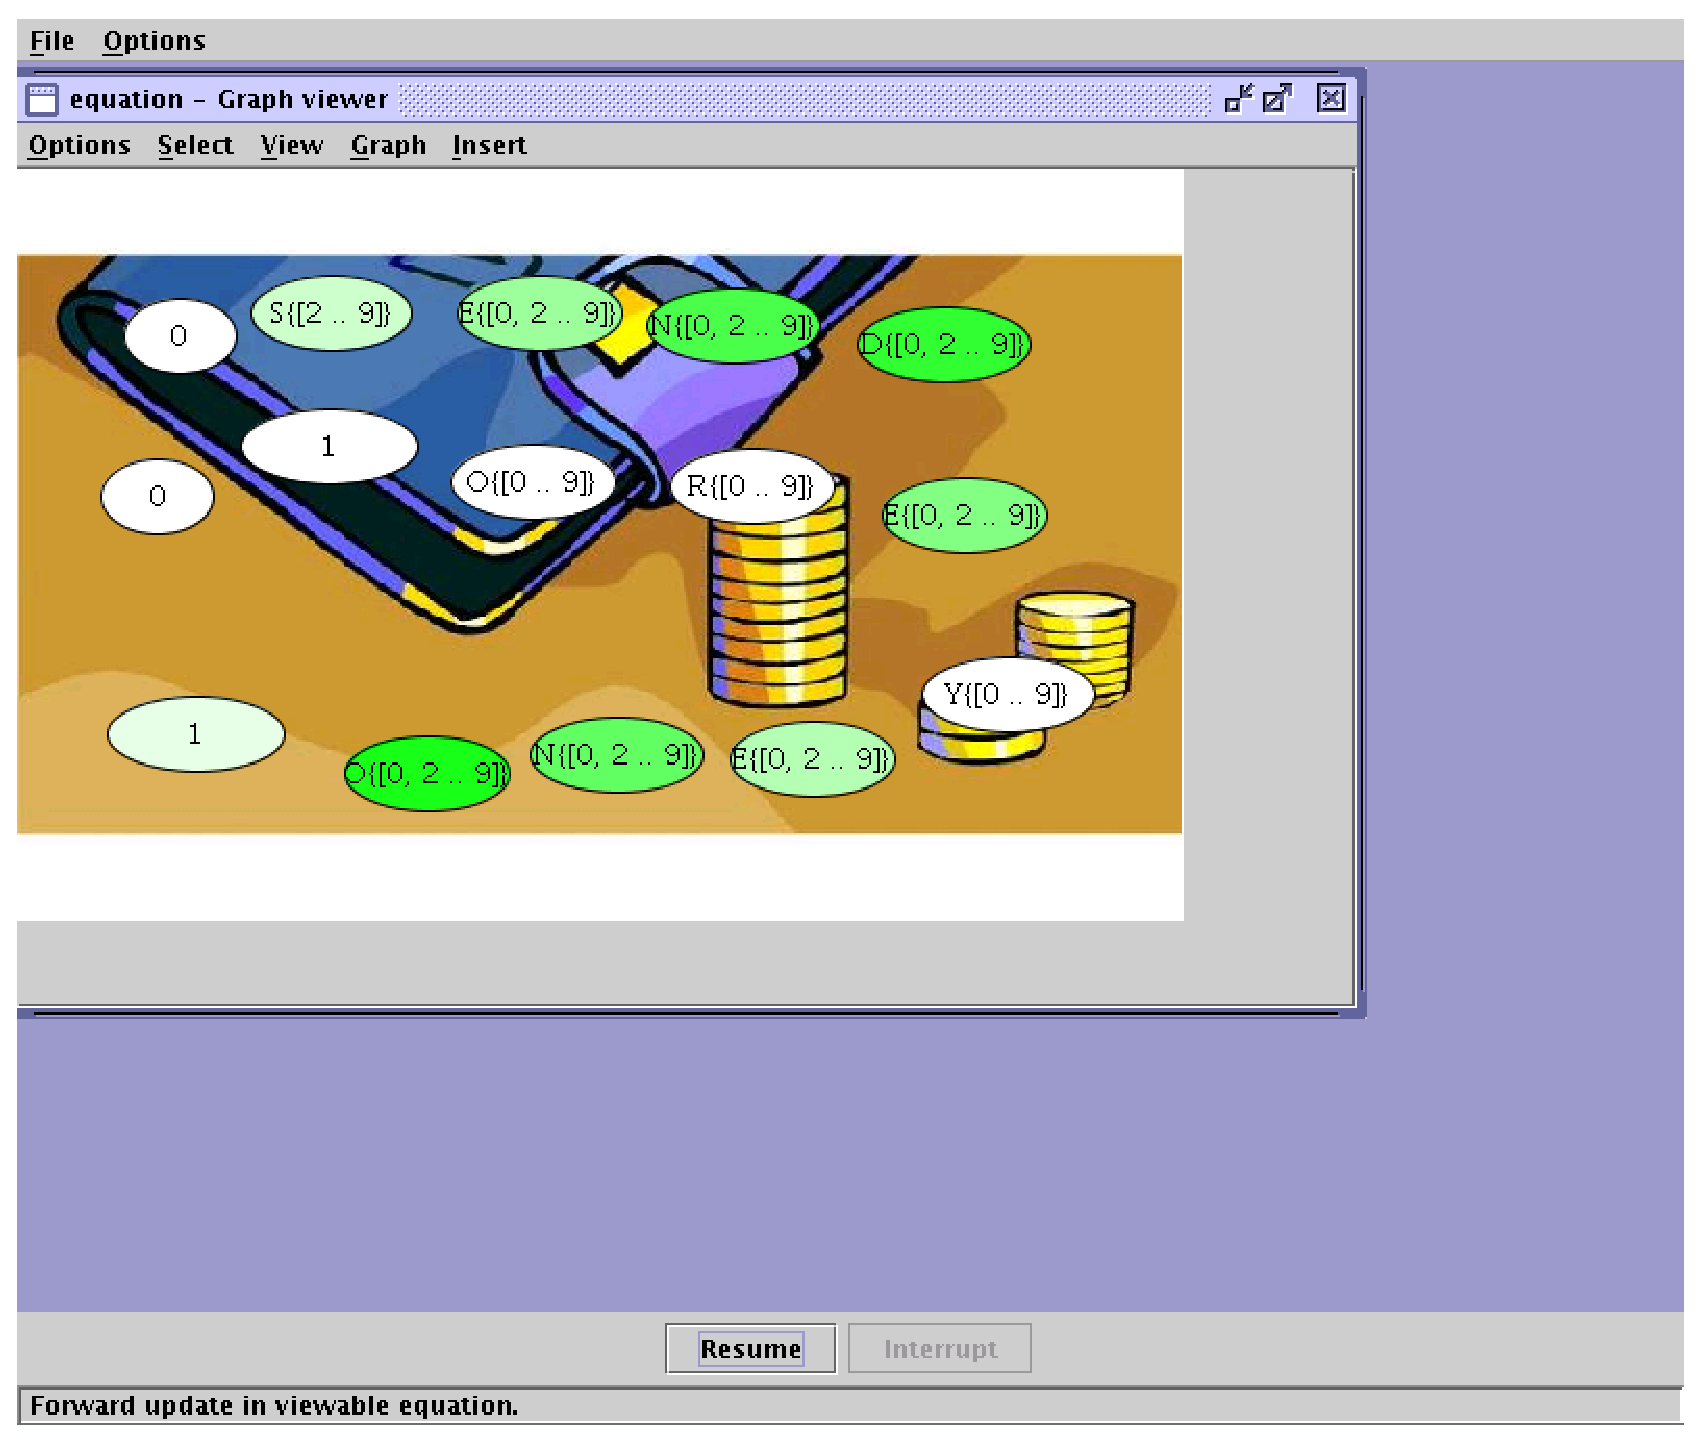
\includegraphics[width=10cm]{vcsendmoremoney}
\caption{The \texttt{SEND+MORE=MONEY} example displayed on a Desktop
\viewer{} with a background image}
\label{fig:sendmoremoney}
\end{figure}

\subsection{Layout}

Items on the desktop may be manually positioned by selecting (single
click) and dragging (click-and-move) them.  New items may be added to
the current selection by holding down the \textbf{Ctrl} key whilst
clicking with the left mouse button.  Ranges of items are selected by
clicking on the background of the desktop and dragging a selection
rectangle around the desired items.  When dragging a selection all
items move, except lines on the \textbf{Network viewer}.

It is also possible to use one of the automatic layout options
available from the \textbf{Graph} menu.  These options make use of the
external graph layout tools \texttt{dot}, \texttt{neato} and
\texttt{twopi} from the AT\&T Labs Research project
\emph{Graphviz}\footnote{\texttt{http://www.research.att.com/sw/tools/graphviz/}}.
These tools should be automatically installed as part of the
{\eclipse} installation procedure.

\subsection{Gantt charts}

The Gantt chart viewer has many of the same options as the Network
viewer previously mentioned but in addition, the \textbf{Gantt} menu
provides access to options that control how transparent the individual
gantt task bars are drawn.  By selecting the \textbf{transparent}
option, regions where tasks overlap will be rendered in a darker
colour.  The darker the colour, the more tasks overlap there.

When either the start time or the duration of a task is a variable,
then the task will be draw as two connected bars indicating the
earliest \& shortest possible occurrence of the task and the latest \&
longest possible occurrence.

Above the gantt chart is a numeric scale indicating time.  By clicking
and dragging this scale can be expanded or shrunk so as to fit the
gantt chart into the window.  This feature works independently of the
zoom.
\begin{figure}[htsp]
\centering
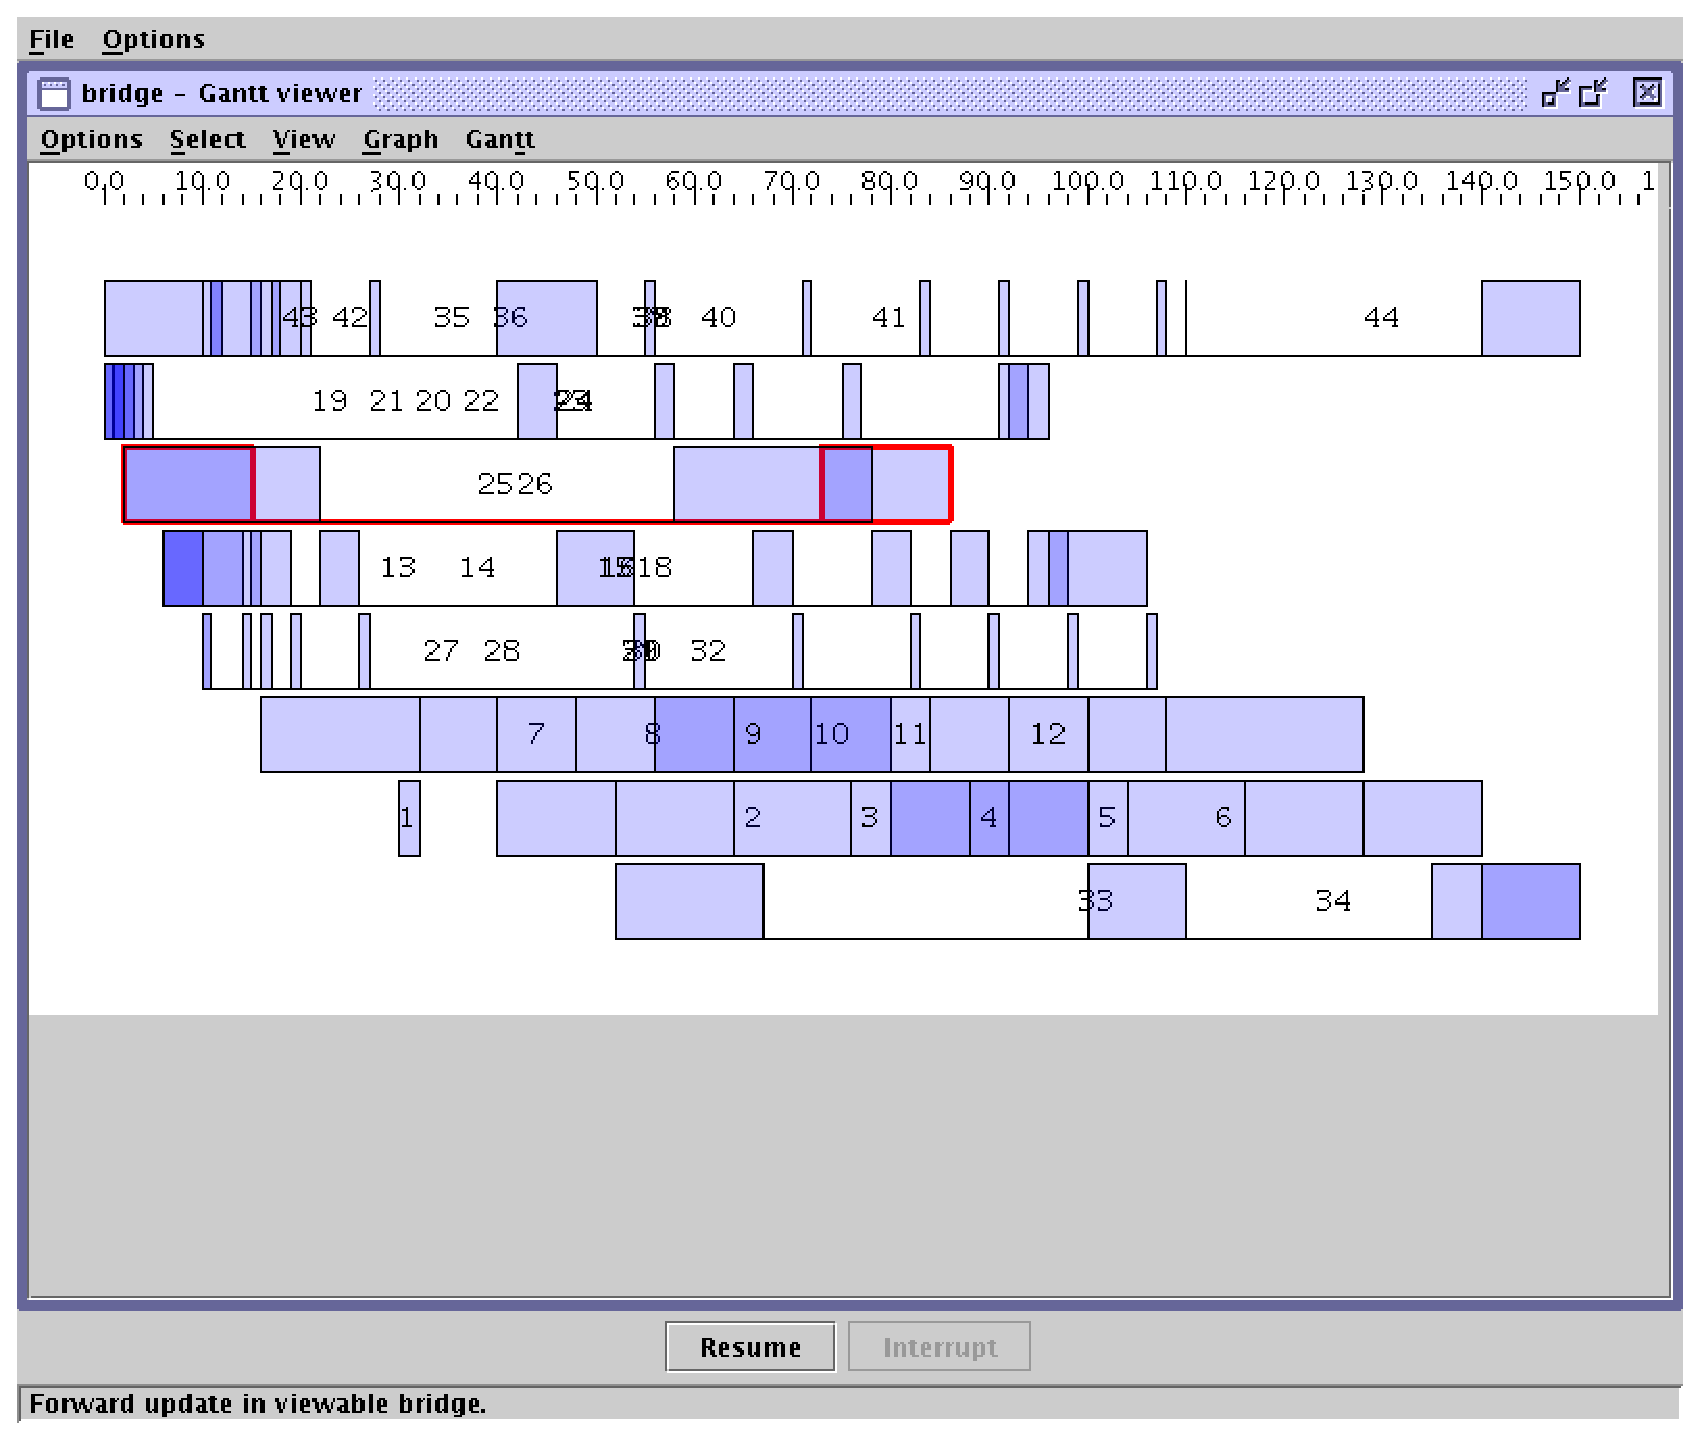
\includegraphics[width=10cm]{vcbridgeexample}
\caption{The VC showing the Gantt viewer for a scheduling
example. Note the highlighted task showing the earliest start/shortest
and latest/longest times of the task.}
\label{fig:bridgeexample}
\end{figure}


\subsection{Printing}

To print the current state of almost all viewers, right-click on the
background and select the \textbf{Print} option from the popup menu.
This will bring up the print dialog as shown in
figure~\ref{fig:printdialog}.

\begin{figure}[htsp]
\centering
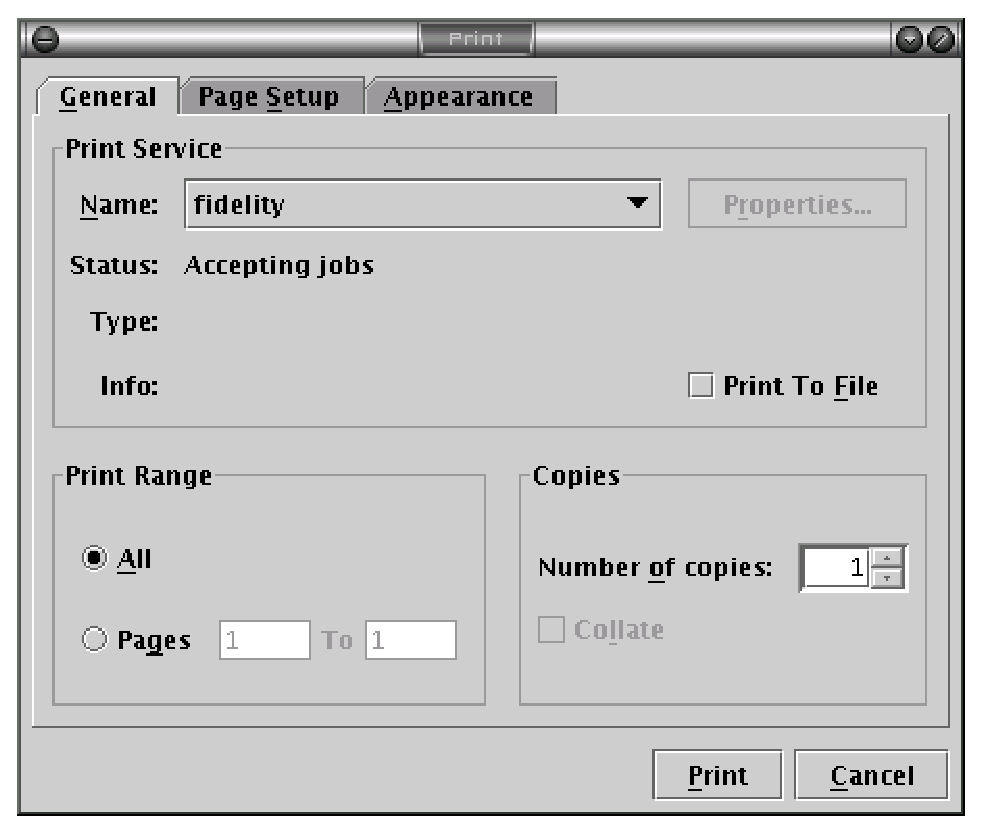
\includegraphics[width=6cm]{vcprintdialog}
\caption{The print options dialog box.}
\label{fig:printdialog}
\end{figure}


\section{Scenarios}
\label{sec:scenarios}

To make the process of setting up the visualisation environment and
the laying out of \viewer{}s and \viewlet{}s quicker, the Java VC
provides a \emph{record and playback} feature where all user visible
changes and actions that are performed following the creation of a
\viewable{} are recorded in a visualisation \textbf{scenario}.  This
action sequence can then be optionally re-played the next time a
\viewable{} of the same name is created.

The common use case is as follows.
\begin{enumerate}
\item Start Java VC.
\item Run program which creates \viewable{} ``foo'' for the first
time.
\item Select \viewer{}s for ``foo''.
\item Arrange \viewer{} windows on screen, resize and scale to taste.
Optionally insert and layout \viewlet{}s on a Desktop viewer.
\item Press \textbf{Resume} button to continue running program.
\item Watch visualisation of program run until \viewable{} is
destroyed (ie. is backtracked over).
\item Re-run program, after having made some changes.
\item Answer \textbf{yes} to the prompt to \emph{reinstate
visualisation preferences for viewable ``foo''}.
\item Watch as things magically re-arrange themselves into the configuration you previously had.
\item (optional) Make some more layout changes.
\item Press \textbf{Resume} again.
\item Repeat.
\end{enumerate}

To make long running visualisation projects easier and also to assist
in running demonstrations, these visualisation preferences can be
saved to disk and loaded back into memory at any time.  The loading
and saving of scenarios is achieved by using the \textbf{Load} and
\textbf{Save} options of the \textbf{File} menu.  The most common
point at which a \textbf{scenario} is saved is just after laying out
all the \viewer{}s and just before passing control back to {\eclipse}.
It should be noted that the scenarios (settings) for many different
viewables can be saved into/loaded from a single file, this is to aid
visualisation of large programs.


\newpage
\printindex

\end{document}
